\documentclass{report}
\setlength{\parskip}{\baselineskip}%
\usepackage{amsmath}
\usepackage{amsfonts,stmaryrd,amssymb} % Math packages

\usepackage{enumerate} % Custom item numbers for enumerations
\usepackage{fontawesome}
\usepackage{setspace}
\usepackage{hyperref}
\usepackage{enumitem}
\usepackage{multicol}
\usepackage{xhfill}
\usepackage[p,osf]{cochineal}
\usepackage[scale=.95,type1]{cabin}
\usepackage[cochineal,bigdelims,cmintegrals,vvarbb]{newtxmath}
\usepackage[zerostyle=c,scaled=.94]{newtxtt}
\usepackage[cal=boondoxo]{mathalfa}
\usepackage[export]{adjustbox}
\usepackage{vwcol}  
\usepackage{fancyhdr}
\DeclareSymbolFont{yhlargesymbols}{OMX}{yhex}{m}{n}
\DeclareMathAccent{\wideparen}{\mathord}{yhlargesymbols}{"F3}

\hypersetup{
	colorlinks=false,
	linkcolor=black,
	filecolor=black,      
	urlcolor=black,
	pdftitle={Overleaf Example},
	pdfpagemode=FullScreen,
	urlbordercolor=white,
}

\urlstyle{same}


	
\newenvironment{cequation}{
	\makeatletter
	\setbool{@fleqn}{false}
	\makeatother
	\begin{equation*}
		}{\end{equation*}}
		
\newcommand{\sol}{\noindent\textbf{Solution:} }
%----------------------------------------------------------------------------------------

\newcommand{\exercise}[1]{%
	\subsection*{\faPencil\ \ Exercise #1\hspace{0.5em}\xrfill[0.175\baselineskip]{1pt}}
}

\newcommand{\practice}[1]{%
	\subsection*{\faFlag\ \ Practice #1\hspace{0.5em}\xrfill[0.175\baselineskip]{1pt}}
}

\newcommand{\revision}[1]{%
	\section*{\faGears\ \ Revision Exercise #1\hspace{0.5em}\xrfill[0.175\baselineskip]{1pt}}
}

\usepackage[ruled]{algorithm2e} % Algorithms

\usepackage[framemethod=tikz]{mdframed} % Allows defining custom boxed/framed environments

\usepackage{listings} % File listings, with syntax highlighting
\lstset{
	basicstyle=\ttfamily, % Typeset listings in monospace font
}

%----------------------------------------------------------------------------------------
%	DOCUMENT MARGINS
%----------------------------------------------------------------------------------------

\usepackage{geometry} % Required for adjusting page dimensions and margins

\geometry{
	paper=a4paper, % Paper size, change to letterpaper for US letter size
	top=2.5cm, % Top margin
	bottom=3cm, % Bottom margin
	left=2.5cm, % Left margin
	right=2.5cm, % Right margin
	headheight=14pt, % Header height
	footskip=1.5cm, % Space from the bottom margin to the baseline of the footer
	headsep=1.2cm, % Space from the top margin to the baseline of the header
	%showframe, % Uncomment to show how the type block is set on the page
}

%----------------------------------------------------------------------------------------
%	FONTS
%----------------------------------------------------------------------------------------

\usepackage[utf8]{inputenc} % Required for inputting international characters
\usepackage[T1]{fontenc} % Output font encoding for international characters

%----------------------------------------------------------------------------------------
%	COMMAND LINE ENVIRONMENT
%----------------------------------------------------------------------------------------

% Usage:
% \begin{commandline}
%	\begin{verbatim}
%		$ ls
%		
%		Applications	Desktop	...
%	\end{verbatim}
% \end{commandline}

\mdfdefinestyle{commandline}{
	leftmargin=10pt,
	rightmargin=10pt,
	innerleftmargin=15pt,
	middlelinecolor=black!50!white,
	middlelinewidth=2pt,
	frametitlerule=false,
	backgroundcolor=black!5!white,
	frametitle={Command Line},
	frametitlefont={\normalfont\sffamily\color{white}\hspace{-1em}},
	frametitlebackgroundcolor=black!50!white,
	nobreak,
}

% Define a custom environment for command-line snapshots
\newenvironment{commandline}{
	\medskip
	\begin{mdframed}[style=commandline]
		}{
	\end{mdframed}
	\medskip
}

%----------------------------------------------------------------------------------------
%	FILE CONTENTS ENVIRONMENT
%----------------------------------------------------------------------------------------

% Usage:
% \begin{file}[optional filename, defaults to "File"]
%	File contents, for example, with a listings environment
% \end{file}

\mdfdefinestyle{file}{
	innertopmargin=1.6\baselineskip,
	innerbottommargin=0.8\baselineskip,
	topline=false, bottomline=false,
	leftline=false, rightline=false,
	leftmargin=2cm,
	rightmargin=2cm,
	singleextra={%
		\draw[fill=black!10!white](P)++(0,-1.2em)rectangle(P-|O);
		\node[anchor=north west]
		at(P-|O){\ttfamily\mdfilename};
		%
		\def\l{3em}
		\draw(O-|P)++(-\l,0)--++(\l,\l)--(P)--(P-|O)--(O)--cycle;
		\draw(O-|P)++(-\l,0)--++(0,\l)--++(\l,0);
	},
	nobreak,
}

% Define a custom environment for file contents
\newenvironment{file}[1][File]{ % Set the default filename to "File"
	\medskip
	\newcommand{\mdfilename}{#1}
	\begin{mdframed}[style=file]
		}{
	\end{mdframed}
	\medskip
}

%----------------------------------------------------------------------------------------
%	NUMBERED QUESTIONS ENVIRONMENT
%----------------------------------------------------------------------------------------

% Usage:
% \begin{question}[optional title]
%	Question contents
% \end{question}

\mdfdefinestyle{question}{
	innertopmargin=1.2\baselineskip,
	innerbottommargin=0.8\baselineskip,
	roundcorner=5pt,
	nobreak,
	singleextra={%
		\draw(P-|O)node[xshift=1em,anchor=west,fill=white,draw,rounded corners=3pt]{%
			\faCaretRight\ \textbf{Example \theQuestion\questionTitle}};
	},
}

\newcounter{Question} % Stores the current question number that gets iterated with each new question

% Define a custom environment for numbered questions
\newenvironment{question}[1][\unskip]{
	\bigskip
	\stepcounter{Question}
	\newcommand{\questionTitle}{~#1}
	\begin{mdframed}[style=question]
		}{
	\end{mdframed}
	\medskip
}

%----------------------------------------------------------------------------------------
%	SOLUTIONS ENVIRONMENT
%----------------------------------------------------------------------------------------

% Usage:
% \begin{solution}
%	Solution contents
% \end{solution}

\mdfdefinestyle{solution}{
	innertopmargin=1.2\baselineskip,
	innerbottommargin=0.8\baselineskip,
	roundcorner=5pt,
	nobreak,
	singleextra={%
		\draw(P-|O)node[xshift=1em,anchor=west,fill=white,draw,rounded corners=5pt]{解};
	},
}

% Define a custom environment for solutions
\newenvironment{solution}{
	\begin{mdframed}[style=solution]
		}{
	\end{mdframed}
}

%----------------------------------------------------------------------------------------
%	WARNING TEXT ENVIRONMENT
%----------------------------------------------------------------------------------------

% Usage:
% \begin{warn}[optional title, defaults to "Warning:"]
%	Contents
% \end{warn}

\mdfdefinestyle{warning}{
	topline=false, bottomline=false,
	leftline=false, rightline=false,
	nobreak,
	singleextra={%
		\draw(P-|O)++(-0.5em,0)node(tmp1){};
		\draw(P-|O)++(0.5em,0)node(tmp2){};
		\fill[black,rotate around={45:(P-|O)}](tmp1)rectangle(tmp2);
		\node at(P-|O){\color{white}\scriptsize\bf !};
		\draw[very thick](P-|O)++(0,-1em)--(O);%--(O-|P);
	}
}

% Define a custom environment for warning text
\newenvironment{warn}[1][Warning:]{ % Set the default warning to "Warning:"
	\medskip
	\begin{mdframed}[style=warning]
		\noindent{\textbf{#1}}
		}{
	\end{mdframed}
	\vspace{-0.5cm}
}

%----------------------------------------------------------------------------------------
%	INFORMATION ENVIRONMENT
%----------------------------------------------------------------------------------------

% Usage:
% \begin{info}[optional title, defaults to "Info:"]
% 	contents
% 	\end{info}

\mdfdefinestyle{info}{%
	topline=false, bottomline=false,
	leftline=false, rightline=false,
	nobreak,
	singleextra={%
		\fill[black](P-|O)circle[radius=0.6em];
		\node at(P-|O){\color{white}\scriptsize\bf \faInfo};
		\draw[very thick](P-|O)++(0,-0.8em)--(O);%--(O-|P);
	}
}

% Define a custom environment for information
\newenvironment{info}[1][Info:]{ % Set the default title to "Info:"
	\medskip
	\begin{mdframed}[style=info]
		\noindent{\textbf{#1}}
		}{
	\end{mdframed}
	\vspace{-0.5cm}
	
}

\mdfdefinestyle{explore}{%
	topline=false, bottomline=false,
	leftline=false, rightline=false,
	nobreak,
	singleextra={%
		\fill[black](P-|O)circle[radius=0.6em];
		\node at(P-|O){\color{white}\scriptsize\bf \faFlask};
		\draw[very thick](P-|O)++(0,-0.8em)--(O);%--(O-|P);
	}
}

% Define a custom environment for warning text
\newenvironment{explore}[1][Exploration Activity:]{ % Set the default warning to "Warning:"
	\medskip
	\begin{mdframed}[style=explore]
		\noindent{\large\textbf{#1}}
		}{
	\end{mdframed}
	\vspace{-0.5cm}
}

\mdfdefinestyle{think}{%
	topline=false, bottomline=false,
	leftline=false, rightline=false,
	nobreak,
	singleextra={%
		\fill[black](P-|O)circle[radius=0.6em];
		\node at(P-|O){\color{white}\scriptsize\bf \faQuestion};
		\draw[very thick](P-|O)++(0,-0.8em)--(O);%--(O-|P);
	}
}

% Define a custom environment for warning text
\newenvironment{think}[1][Think about It:]{ % Set the default warning to "Warning:"
	\medskip
	\begin{mdframed}[style=think]
		\noindent{\large\textbf{#1}}
		}{
	\end{mdframed}
	\vspace{-0.5cm}
}



\usepackage{tabularx}
\usepackage{hlist}
\usepackage{tasks}
\usepackage{tabularray}
\usepackage{multirow}
\newcolumntype{Y}{>{\centering\arraybackslash}X}

\allowdisplaybreaks

\begin{document}
\pagestyle{fancy}
%... then configure it.
\fancyhead{} % clear all header fields
\fancyhead[RO,LE]{\thepage}
\fancyhead[LO,RE]{\leftmark}
\fancyfoot{} % clear all footer fields

\fancyfoot[LO,RE]{Dong Zong Addmath Textbook Senior 1 Volume II}
\fancyfoot[RO,RE]{\thepage}

\onehalfspacing
\setcounter{chapter}{10}

\chapter{Trigonometric Identities and Trigonometric Equations}

\section{Basic Relationships of Trigonometric Functions of the Same Angle}

\subsection*{Reciprocal Relationships}
$\begin{aligned} \sin \theta \cdot \operatorname{cosec} \theta & =\dfrac{y}{r} \cdot \dfrac{r}{y}=1 \\ \cos \theta \cdot \sec \theta & =\dfrac{x}{r} \cdot \dfrac{r}{x}=1 \\ \tan \theta \cdot \cot \theta & =\dfrac{y}{x} \cdot \dfrac{x}{y}=1\end{aligned}$

\noindent That is,
\begin{info}[Reciprocal Relationships]
	
	$\begin{aligned} \operatorname{cosec} \theta&=\dfrac{1}{\sin \theta} \\ \sec \theta&=\dfrac{1}{\cos \theta} \\ \cot \theta&=\dfrac{1}{\tan \theta}\end{aligned}$
\end{info}

\subsection*{Quotient Relationships}
$\begin{aligned} & \dfrac{\sin \theta}{\cos \theta}=\dfrac{\dfrac{y}{r}}{\dfrac{x}{r}}=\dfrac{y}{x}=\tan \theta \\ & \dfrac{\cos \theta}{\sin \theta}=\dfrac{\dfrac{x}{r}}{\dfrac{y}{r}}=\dfrac{x}{y}=\cot \theta\end{aligned}$

\noindent That is,
\begin{info}[Quotient Relationships]
	
	$\begin{aligned} \tan \theta&=\dfrac{\sin \theta}{\cos \theta} \\ \cot \theta&=\dfrac{\cos \theta}{\sin \theta}\end{aligned}$
\end{info}

\subsection*{Square Relationships}

\begin{multicols}{2}
	Because$\qquad$
	$
	\begin{aligned}[t]
		\sin ^2 \theta+\cos ^2 \theta & =\left(\dfrac{y}{r}\right)^2+\left(\dfrac{x}{r}\right)^2 \\
		                              & =\dfrac{x^2+y^2}{r^2}                                    
	\end{aligned}
	$
	
	\noindent On a Cartesian plane, as shown in the figure to the right,
	\begin{flalign*}
		&&x^2+y^2=r^2&&&&&&&&\\
		\text{Hence}&&\sin ^2 \theta+\cos ^2 \theta & =\dfrac{r^2}{r^2} &&\\
		&& & =1 &
	\end{flalign*}
	\noindent Dividing both sides of $\sin ^2 \theta+\cos ^2 \theta=1$ by $\cos ^2 \theta$, we get
	\begin{align*}
		\dfrac{\sin ^2 \theta}{\cos ^2 \theta}+\dfrac{\cos ^2 \theta}{\cos ^2 \theta} & =\dfrac{1}{\cos ^2 \theta} \\
		\tan ^2 \theta+1 & =\sec ^2 \theta &   &   &   &   
	\end{align*}
	Dividing both sides of $\sin ^2 \theta+\cos ^2 \theta=1$ by $\sin ^2 \theta$, 得
	\begin{align*}
		\dfrac{\sin ^2 \theta}{\sin ^2 \theta}+\dfrac{\cos ^2 \theta}{\sin ^2 \theta} & =\dfrac{1}{\sin ^2 \theta} \\
		1+\cot ^2 \theta & =\operatorname{cosec}^2 \theta &   &   &   &   
	\end{align*}
	\columnbreak
	
	\begin{center}
		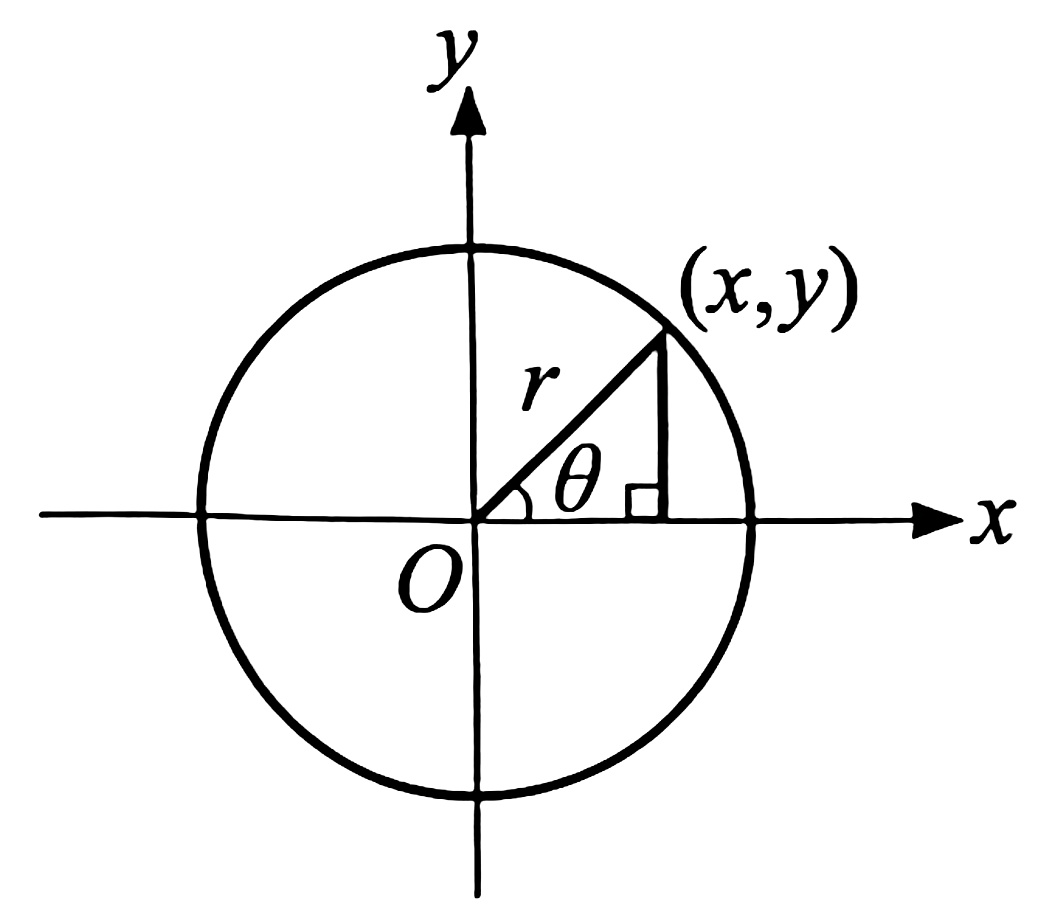
\includegraphics[width=0.25\textwidth]{assets/11-1.jpg}
	\end{center}
\end{multicols}
\vspace{-4em}
\noindent That is,
\begin{info}[Square Relationships]
	
	$\begin{aligned} & \sin ^2 \theta+\cos ^2 \theta=1 \\ & 1+\tan ^2 \theta=\sec ^2 \theta \\ & 1+\cot ^2 \theta=\operatorname{cosec}^2 \theta\end{aligned}$
\end{info}

An equation where both sides hold true for defined conditions is called an identity, and an identity containing trigonometric functions is called a \textbf{trigonometric identity}. By utilizing these identities, trigonometric expressions can be simplified or other trigonometric identities can be proven.
\begin{think}
	
	\noindent Under what circumstances does the following equation not hold?
	\begin{tasks}[label=\arabic*.](2)
		\task $\tan \theta=\dfrac{\sin \theta}{\cos \theta}$
		\task $\cot \theta=\dfrac{\cos \theta}{\sin \theta}$
		\task $1+\tan ^2 \theta=\sec ^2 \theta$
		\task $1+\cot ^2 \theta=\operatorname{cosec}^2 \theta$
	\end{tasks}
\end{think}

\begin{question}
	Simplify the following expressions:
	\vspace{-1em}
	\begin{enumerate}[label=(\alph*)]
		\item $(\sin A+\cos A)^2+(\sin A-\cos A)^2$
		\item $\operatorname{cosec} \theta \cdot \tan \theta \cdot \sec \theta \cdot \sin \theta \cdot \cos \theta$
	\end{enumerate}
	
	\sol{}
	\vspace{-1em}
	\begin{enumerate}[label=(\alph*)]
		\item $\begin{aligned}[t] & (\sin A+\cos A)^2+(\sin A-\cos A)^2 \\ & =\sin ^2 A+2 \sin A \cos A+\cos ^2 A+\sin ^2 A-2 \sin A \cos A+\cos ^2 A \\ & =2\left(\sin ^2 A+\cos ^2 A\right) \\ & =2\end{aligned}$
		\item $\begin{aligned}[t] & \operatorname{cosec} \theta \cdot \tan \theta \cdot \sec \theta \cdot \sin \theta \cdot \cos \theta \\ & =\dfrac{1}{\sin \theta} \cdot \dfrac{\sin \theta}{\cos \theta} \cdot \dfrac{1}{\cos \theta} \cdot \sin \theta \cdot \cos \theta \\ & =\dfrac{\sin \theta}{\cos \theta} \\ & =\tan \theta\end{aligned}$
	\end{enumerate}
\end{question}

\practice{11.1a}
Simplify the following expressions:
\begin{tasks}[label=\arabic*.](2)
	\task $\left(1+\tan ^2 \theta\right) \cos ^2 \theta$
	\task $\sec ^2 A-\tan ^2 A-\sin ^2 A$
	\task $\dfrac{2 \cos ^2 \theta-1}{1-2 \sin ^2 \theta}$
	\task $\operatorname{cosec}^2 \alpha-\tan \alpha \cot \alpha$
\end{tasks}

\begin{question}
	Prove that $\dfrac{1}{1+\sin ^2 \theta}+\dfrac{1}{1+\operatorname{cosec}^2 \theta}=1$.
	
	\proof{}
	
	\noindent $\begin{aligned} \dfrac{1}{1+\sin ^2 \theta}+\dfrac{1}{1+\operatorname{cosec}^2 \theta} & =\dfrac{1}{1+\sin ^2 \theta}+\dfrac{1}{1+\dfrac{1}{\sin ^2 \theta}} \\ & =\dfrac{1}{1+\sin ^2 \theta}+\dfrac{\sin ^2 \theta}{\sin ^2 \theta+1} \\ & =\dfrac{1+\sin ^2 \theta}{1+\sin ^2 \theta} \\ & =1\end{aligned}$
\end{question}

\begin{question}
	Prove that $\sin ^4 A+\sin ^2 A \cos ^2 A+\cos ^2 A=1$.
	
	\proof{}
	
	\noindent $\begin{aligned} \sin ^4 A+\sin ^2 A \cos ^2 A+\cos ^2 A & =\sin ^2 A\left(\sin ^2 A+\cos ^2 A\right)+\cos ^2 A \\ & =\sin ^2 A+\cos ^2 A \\ & =1\end{aligned}$
\end{question}

\begin{question}
	Prove that $\dfrac{1}{\sec \theta-\tan \theta}=\sec \theta+\tan \theta$.
	
	\proof{}
	
	\noindent $\begin{aligned} \dfrac{1}{\sec \theta-\tan \theta} & =\dfrac{1}{\dfrac{1}{\cos \theta}-\dfrac{\sin \theta}{\cos \theta}} \\ & =\dfrac{\cos \theta}{1-\sin \theta} \\ & =\dfrac{\cos \theta}{1-\sin \theta} \cdot \dfrac{1+\sin \theta}{1+\sin \theta} \\ & =\dfrac{\cos \theta(1+\sin \theta)}{1-\sin ^2 \theta} \\ & =\dfrac{\cos \theta(1+\sin \theta)}{\cos ^2 \theta} \\ & =\sec \theta+\tan \theta\end{aligned}$
\end{question}

\begin{question}
	Prove that $\dfrac{\cos ^2 \theta+\tan ^2 \theta-1}{\sin ^2 \theta}=\tan ^2 \theta$.
	
	\proof{}
	
	\noindent $\begin{aligned} \dfrac{\cos ^2 \theta+\tan ^2 \theta-1}{\sin ^2 \theta} & =\dfrac{\cos ^2 \theta+\tan ^2 \theta-\left(\sin ^2 \theta+\cos ^2 \theta\right)}{\sin ^2 \theta} \\ & =\dfrac{\tan ^2 \theta}{\sin ^2 \theta}-\dfrac{\sin ^2 \theta}{\sin ^2 \theta} \\ & =\dfrac{\sin ^2 \theta}{\cos ^2 \theta} \cdot \dfrac{1}{\sin ^2 \theta}-1 \\ & =\sec ^2 \theta-1 \\ & =\tan ^2 \theta\end{aligned}$
\end{question}

\begin{question}
	Prove that $\dfrac{1-2 \cos ^2 A}{\sin A \cos A}=\tan A-\cot A 。$.
	
	\begin{enumerate}[label=\textbf{Approach (\arabic*)}, leftmargin=*, labelsep=1.5em]
		\item $\begin{aligned}[t] \dfrac{1-2 \cos ^2 A}{\sin A \cos A} & =\dfrac{1-\cos ^2 A-\cos ^2 A}{\sin A \cos A} \\ & =\dfrac{\sin ^2 A-\cos ^2 A}{\sin A \cos A} \\ & =\dfrac{\sin ^2 A}{\sin A \cos A}-\dfrac{\cos ^2 A}{\sin A \cos A} \\ & =\tan A-\cot A\end{aligned}$
		\item $\begin{aligned}[t] \tan A-\cot A & =\dfrac{\sin A}{\cos A}-\dfrac{\cos A}{\sin A} \\ & =\dfrac{\sin ^2 A-\cos ^2 A}{\sin A \cos A} \\ & =\dfrac{1-\cos ^2 A-\cos ^2 A}{\sin A \cos A} \\ & =\dfrac{1-2 \cos ^2 A}{\sin A \cos A}\end{aligned}$
	\end{enumerate}
\end{question}
\begin{question}
	Prove that $\cot ^2 \theta+\cot ^4 \theta=\operatorname{cosec}^4 \theta-\operatorname{cosec}^2 \theta$.
	
	\proof{}
	    
	\noindent L.H.S. $\begin{aligned}[t] \cot ^2 \theta+\cot ^4 \theta & =\cot ^2 \theta\left(1+\cot ^2 \theta\right) \\ & =\dfrac{\cos ^2 \theta}{\sin ^2 \theta} \cdot\left(1+\dfrac{\cos ^2 \theta}{\sin ^2 \theta}\right) \\ & =\dfrac{\cos ^2 \theta}{\sin ^2 \theta} \cdot\left(\dfrac{\sin ^2 \theta+\cos ^2 \theta}{\sin ^2 \theta}\right) \\ & =\dfrac{\cos ^2 \theta}{\sin ^4 \theta}\end{aligned}$
	
	\noindent R.H.S. $\begin{aligned}[t]\operatorname{cosec}^4 \theta-\operatorname{cosec}^2 \theta&=\operatorname{cosec}^2 \theta\left(\operatorname{cosec}^2 \theta-1\right)\\
	& =\dfrac{1}{\sin ^2 \theta} \cdot\left(\dfrac{1}{\sin ^2 \theta}-1\right) \\
	& =\dfrac{1}{\sin ^2 \theta} \cdot\left(\dfrac{1-\sin ^2 \theta}{\sin ^2 \theta}\right) \\
	& =\dfrac{1}{\sin ^2 \theta} \cdot\left(\dfrac{\cos ^2 \theta}{\sin ^2 \theta}\right) \\
	& =\dfrac{\cos ^2 \theta}{\sin ^4 \theta}
	\end{aligned}
	$
	
	\noindent $\therefore$ $\cot ^2 \theta+\cot ^4 \theta=\operatorname{cosec}^4 \theta-\operatorname{cosec}^2 \theta$
\end{question}

\newpage
Trigonometric identities can be proven by starting from either side of the equation and simplifying it to match the other side (as in Example 6). Alternatively, both sides of the equation can be simplified to match a common expression (as in Example 7), thereby proving the trigonometric identity.

\practice{11.1b}
Prove the following identities:
\begin{tasks}[label=\arabic*.](2)
	\task $\sec x-\cos x=\sin x \tan x$
	\task $\left(1-\sin ^2 \theta\right)\left(1+\tan ^2 \theta\right)=1$
	\task $\sin ^2 \theta \cos ^2 \theta=\dfrac{1}{\sec ^2 \theta+\operatorname{cosec}^2 \theta}$
\end{tasks}

\exercise{11.1}
Simplify the following expressions (Questions 1-4):
\begin{tasks}[label=\arabic*.](2)
	\task $\dfrac{\tan \theta+\cot \theta}{\sec \theta \operatorname{cosec} \theta}$
	\task $\dfrac{1-\cos ^2 \alpha}{1-\sin ^2 \alpha}+\cos \alpha \sec \alpha$
	\task $\dfrac{\sin A+\cos A}{\sec A+\operatorname{cosec} A}$
	\task $\cos ^2 \alpha \operatorname{cosec}^2 \alpha+\sin ^2 \alpha+\cos ^2 \alpha$
\end{tasks}

\noindent Prove the following identities (Questions 5-15):
\begin{tasks}[label=\arabic*.,start=5]
	\task $(1+\tan A)^2+(1-\tan A)^2=2 \sec ^2 A$
	\task $\sec ^2 \theta+\operatorname{cosec}^2 \theta=\sec ^2 \theta \operatorname{cosec}^2 \theta$
	\task $\sin A \cos A=\dfrac{1}{\tan A+\cot A}$
	\task $\sec ^4 \theta-\sec ^2 \theta=\tan ^4 \theta+\tan ^2 \theta$
	\task $\left(1-\sin ^2 \theta\right)\left(\sec ^2 \theta-1\right)=\sin ^2 \theta$
	\task $\sin A(1+\tan A)+\cos A(1+\cot A)=\sec A+\operatorname{cosec} A$
	\task $(\tan \theta+\cot \theta)^2=\sec ^2 \theta+\operatorname{cosec}^2 \theta$
	\task $\dfrac{\tan A+\cot B}{\cot A+\tan B}=\dfrac{\tan A}{\tan B}$
	\task $\dfrac{1+\tan ^2 A}{1+\cot ^2 A}=\left(\dfrac{1-\tan A}{1-\cot A}\right)^2$
	\task $\dfrac{\tan A \sin A}{\tan A-\sin A}=\dfrac{\tan A+\sin A}{\tan A \sin A}$
	\task $\dfrac{2 \sin A \cos A-\cos A}{1-\sin A+\sin ^2 A-\cos ^2 A}=\cot A$
\end{tasks}

\section{Trigonometric Functions of Sums and Differences of Angles}

Now, let's take a look at the relationship between the trigonometric values of the sum and difference of two angles and the trigonometric values of the individual angles.

\subsection*{Cosine of the Sum and Difference of Two Angles}

\begin{center}
	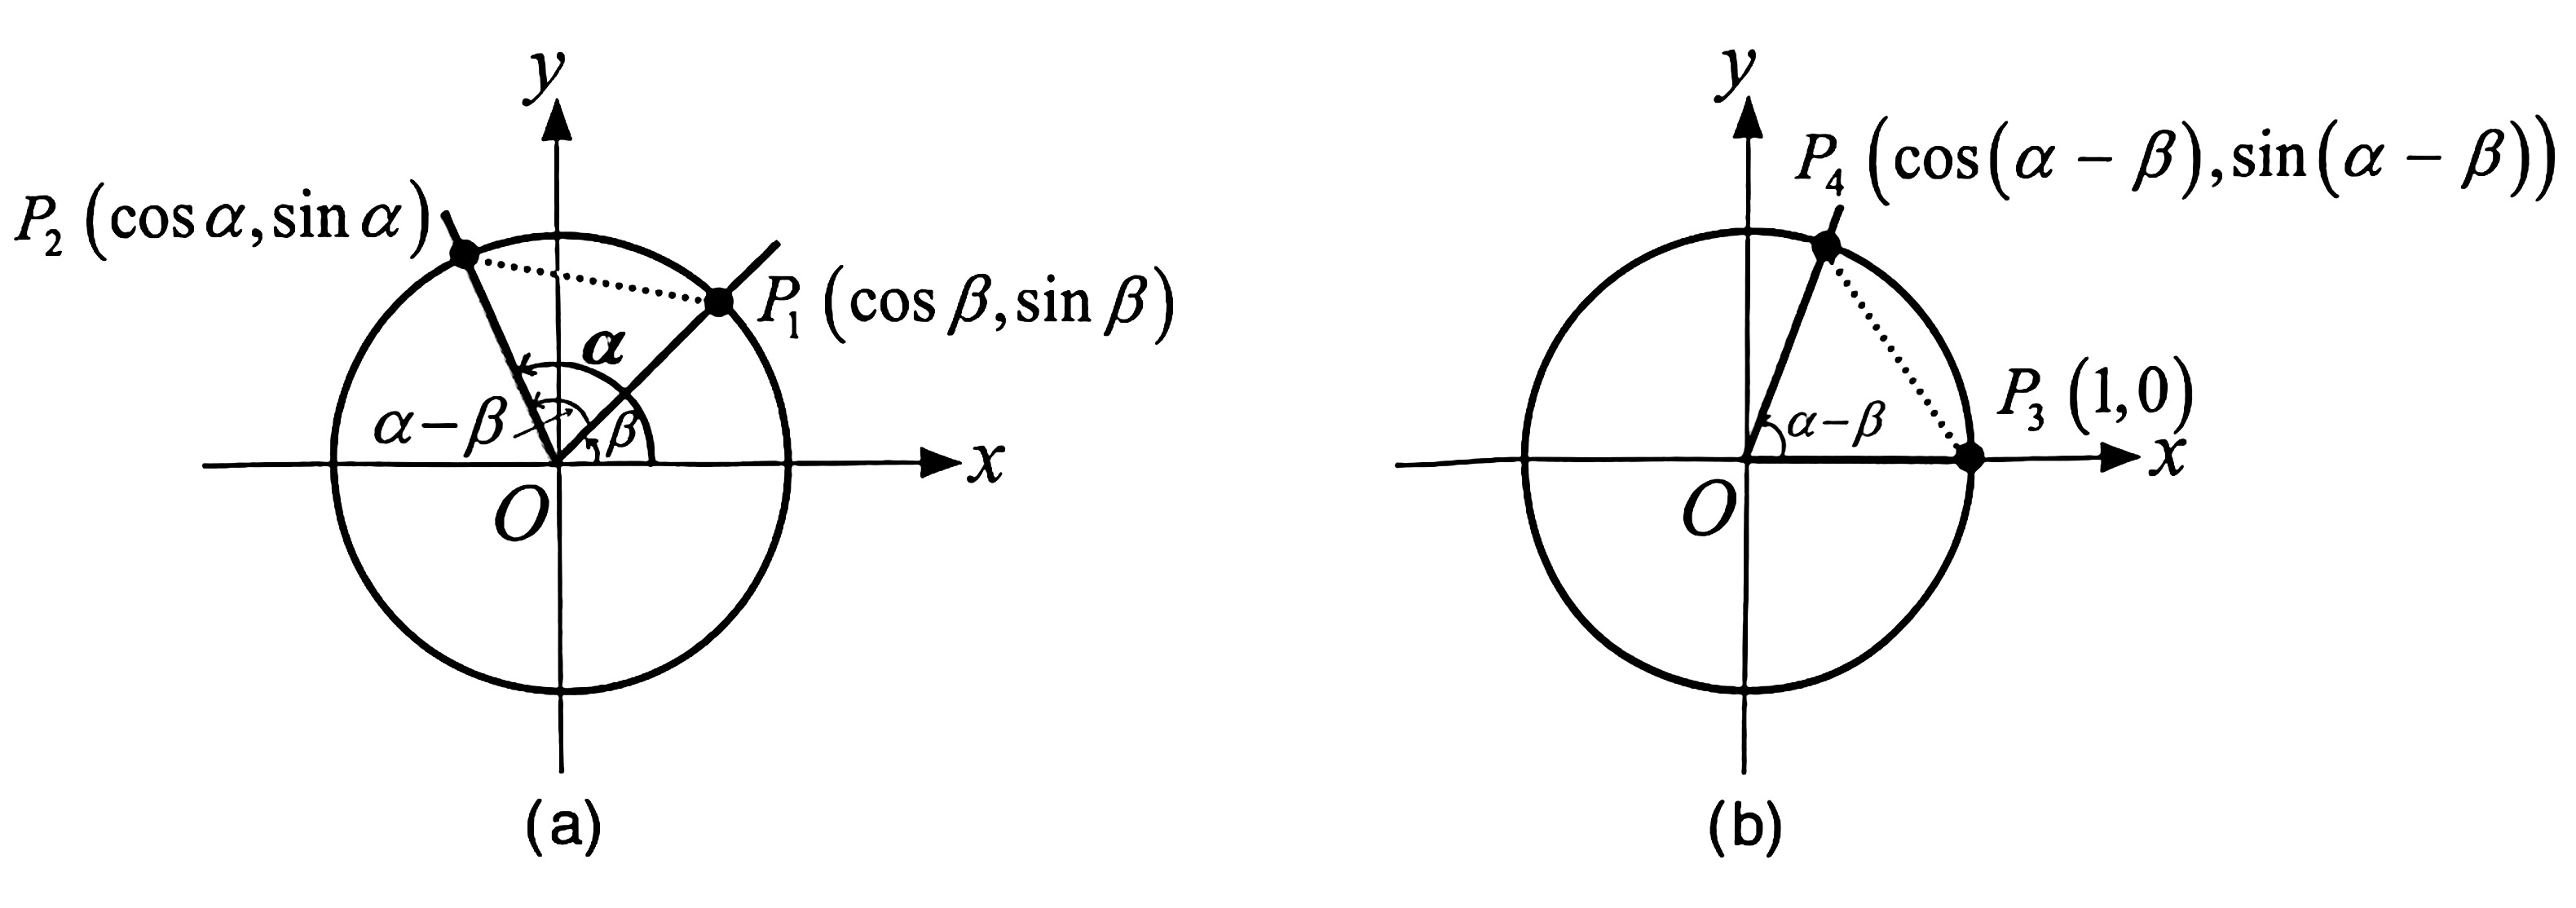
\includegraphics[width=0.8\textwidth]{assets/11-2.jpg}
\end{center}
\vspace{-2em}
As shown in left figure above, consider the unit circle with the origin \( O \) as its center. Let \( \beta \) be an angle whose terminal side intersects the circle at point \( P_1 \), and let \( \alpha \) be an angle whose terminal side intersects the circle at point \( P_2 \). The coordinates of point \( P_1 \) and point \( P_2 \) are \( P_1(\cos \beta, \sin \beta) \) and \( P_2(\cos \alpha, \sin \alpha) \), respectively.

\noindent From the left figure above, $\begin{aligned}[t]\left|P_1 P_2\right| & =\sqrt{(\cos \alpha-\cos \beta)^2+(\sin \alpha-\sin \beta)^2} \\ & =\sqrt{\cos ^2 \alpha-2 \cos \alpha \cos \beta+\cos ^2 \beta+\sin ^2 \alpha-2 \sin \alpha \sin \beta+\sin ^2 \beta} \\ & =\sqrt{2-2 \cos \alpha \cos \beta-2 \sin \alpha \sin \beta}\end{aligned}$

Rotate \( \Delta O P_1 P_2 \) clockwise so that \( O P_1 \) lies on the positive \( x \)-axis, which yields \( \triangle O P_3 P_4 \), as shown in right figure above. Now, the coordinates of point \( P_3 \) and point \( P_4 \) are \( P_3(1,0) \) and \( P_4(\cos (\alpha-\beta), \sin (\alpha-\beta)) \), respectively.

\noindent From the right figure above, $\begin{aligned}[t]\left|P_3 P_4\right| & =\sqrt{(\cos (\alpha-\beta)-1)^2+(\sin (\alpha-\beta)-0)^2} \\ & =\sqrt{\cos ^2(\alpha-\beta)-2 \cos (\alpha-\beta)+1+\sin ^2(\alpha-\beta)} \\ & =\sqrt{2-2 \cos (\alpha-\beta)}\end{aligned}$

By applying the property of congruence between \( \triangle O P_1 P_2 \) and \( \triangle O P_3 P_4 \), namely \( |P_1 P_2| = |P_3 P_4| \), we can derive the cosine formulas for the sum and difference of two angles.
\begin{align*}
	\sqrt{2-2 \cos \alpha \cos \beta-2 \sin \alpha \sin \beta} & =\sqrt{2-2 \cos (\alpha-\beta)} \\ 2-2 \cos \alpha \cos \beta-2 \sin \alpha \sin \beta & =2-2 \cos (\alpha-\beta) \\ 2 \cos (\alpha-\beta) & =2 \cos \alpha \cos \beta+2 \sin \alpha \sin \beta
\end{align*}

\vspace{-2.5em}
We get
\begin{info}[Cosine of the Sum of Two Angles]
	
	$\cos (\alpha+\beta)=\cos \alpha \cos \beta-\sin \alpha \sin \beta$
\end{info}

Replacing \( \beta \) with \( -\beta \) in the cosine formula for the sum of two angles,    
\begin{align*}
	\cos [\alpha-(-\beta)]=\cos \alpha \cos (-\beta)+\sin \alpha \sin (-\beta) 
\end{align*}

\vspace{-2.5em}
We get
\begin{info}[Cosine of the Difference of Two Angles]
	
	$\cos (\alpha-\beta)=\cos \alpha \cos \beta+\sin \alpha \sin \beta$
\end{info}

\subsection*{Sine of the Sum and Difference of Two Angles}

The sine formulas for the sum and difference of two angles can be derived from the complementary angle relationship of trigonometric functions.

\noindent $\begin{aligned} \sin (\alpha-\beta) & =\cos \left[\dfrac{\pi}{2}-(\alpha-\beta)\right] \\ & =\cos \left[\left(\dfrac{\pi}{2}-\alpha\right)+\beta\right] \\ & =\cos \left(\dfrac{\pi}{2}-\alpha\right) \cos \beta-\sin \left(\dfrac{\pi}{2}-\alpha\right) \sin \beta\end{aligned}$

\noindent We get
\begin{info}[Sine of the Sum of Two Angles]
	
	$\sin (\alpha+\beta)=\sin \alpha \cos \beta+\cos \alpha \sin \beta$
\end{info}

Replacing \( \beta \) with \( -\beta \) in the sine formula for the sum of two angles,
\begin{align*}
	\sin [\alpha-(-\beta)]=\sin \alpha \cos (-\beta)+\cos \alpha \sin (-\beta) 
\end{align*}

\vspace{-2em}
\noindent We get
\begin{info}[Sine of the Difference of Two Angles]
	
	$\sin (\alpha-\beta)=\sin \alpha \cos \beta-\cos \alpha \sin \beta$
\end{info}

\begin{question}
	Without using a calculator, find the values of the following trigonometric expressions:
	\begin{tasks}[label=(\alph*)](2)
		\task $\cos 15^{\circ}$
		\task $\sin \dfrac{7 \pi}{12}$
	\end{tasks}
	    
	\sol{}
	\begin{enumerate}[label=(\alph*)]
		\item $\begin{aligned}[t] \cos 15^{\circ} & =\cos \left(45^{\circ}-30^{\circ}\right) \\ & =\cos 45^{\circ} \cos 30^{\circ}+\sin 45^{\circ} \sin 30^{\circ} \\ & =\dfrac{\sqrt{2}}{2} \cdot \dfrac{\sqrt{3}}{2}+\dfrac{\sqrt{2}}{2} \cdot \dfrac{1}{2} \\ & =\dfrac{\sqrt{6}+\sqrt{2}}{4}\end{aligned}$
		\item $\begin{aligned}[t] \sin \dfrac{7 \pi}{12} & =\sin \left(\dfrac{\pi}{3}+\dfrac{\pi}{4}\right) \\ & =\sin \dfrac{\pi}{3} \cos \dfrac{\pi}{4}+\cos \dfrac{\pi}{3} \sin \dfrac{\pi}{4} \\ & =\dfrac{\sqrt{3}}{2} \cdot \dfrac{\sqrt{2}}{2}+\dfrac{1}{2} \cdot \dfrac{\sqrt{2}}{2} \\ & =\dfrac{\sqrt{6}+\sqrt{2}}{4}\end{aligned}$
	\end{enumerate}
\end{question}

\begin{question}
	Without using a calculator, find the value of $\cos 70^{\circ} \cos 20^{\circ}-\sin 70^{\circ} \sin 20^{\circ}$.
	
	\sol{}
	    
	\noindent $\begin{aligned} \cos 70^{\circ} \cos 20^{\circ}-\sin 70^{\circ} \sin 20^{\circ} & =\cos \left(70^{\circ}+20^{\circ}\right) \\ & =\cos 90^{\circ} \\ & =0\end{aligned}$
\end{question}

\begin{think}
	    
	\noindent Are $\cos \left(45^{\circ}-30^{\circ}\right)$ and $\cos 45^{\circ}-\cos 30^{\circ}$ the same?
\end{think}

\begin{question}
	Prove that $\cos 4 A \cos A+\sin 4 A \sin A=\cos 2 A \cos A-\sin 2 A \sin A$.
	
	\proof{}
	
	\noindent $\begin{aligned} & \cos 4 A \cos A+\sin 4 A \sin A \\ & =\cos (4 A-A) \\ & =\cos 3 A \\ & =\cos (2 A+A) \\ & =\cos 2 A \cos A-\sin 2 A \sin A\end{aligned}$
\end{question}

\begin{question}
	Prove that $\cos \theta+\sqrt{3} \sin \theta=2 \sin \left(\dfrac{\pi}{6}+\theta\right)$.
	
	\proof{}
	    
	\noindent $\begin{aligned} 2 \sin \left(\dfrac{\pi}{6}+\theta\right) & =2\left(\sin \dfrac{\pi}{6} \cos \theta+\cos \dfrac{\pi}{6} \sin \theta\right) \\ & =2\left(\dfrac{1}{2} \cos \theta+\dfrac{\sqrt{3}}{2} \sin \theta\right) \\ & =\cos \theta+\sqrt{3} \sin \theta\end{aligned}$
\end{question}

\newpage
\practice{11.2a}
\begin{enumerate}
	\item Without using a calculator, find the values of the following trigonometric expressions:
	      \begin{tasks}[label=(\alph*)](2)
	      	\task $\cos 75^{\circ}$
	      	\task $\sin \left(-\dfrac{5 \pi}{12}\right)$
	      	\task $\cos 80^{\circ} \cos 20^{\circ}+\sin 80^{\circ} \sin 20^{\circ}$
	      	\task $\sin 13^{\circ} \cos 17^{\circ}+\cos 13^{\circ} \sin 17^{\circ}$
	      \end{tasks}
	\item Prove that $\cos \theta-\sin \theta=\sqrt{2} \cos \left(45^{\circ}+\theta\right)$ 。
	\item Prove that $\cos (A+B)-\cos (A-B)=-2 \sin A \sin B$ 。
	\item Prove that $\sin (A+B)+\sin (A-B)=2 \sin A \cos B$ 。
\end{enumerate}

\subsection*{Tangent of the Sum and Difference of Two Angles}

By applying the relationship between tangent as the ratio of sine to cosine, we can obtain the tangent formulas for the sum and difference of two angles.
\begin{align*}
	\tan (\alpha+\beta)= & \dfrac{\sin (\alpha+\beta)}{\cos (\alpha+\beta)} \\ & =\dfrac{\sin \alpha \cos \beta+\cos \alpha \sin \beta}{\cos \alpha \cos \beta-\sin \alpha \sin \beta} \\ & =\dfrac{\dfrac{\sin \alpha \cos \beta+\cos \alpha \sin \beta}{\cos \alpha \cos \beta}}{\dfrac{\cos \alpha \cos \beta-\sin \alpha \sin \beta}{\cos \alpha \cos \beta}}
\end{align*}
We get
\begin{info}[Tangent of the Sum of Two Angles]
	
	$\tan (\alpha+\beta)=\dfrac{\tan \alpha+\tan \beta}{1-\tan \alpha \tan \beta}$
\end{info}

Replacing \( \beta \) with \( -\beta \) in the tangent formula for the sum of two angles,
\begin{align*}
	\tan (\alpha-\beta)=\dfrac{\tan \alpha-\tan \beta}{1+\tan \alpha \tan \beta} 
\end{align*}

We get
\begin{info}[Tangent of the Difference of Two Angles]
	
	$\tan (\alpha-\beta)=\dfrac{\tan \alpha-\tan \beta}{1+\tan \alpha \tan \beta}$
\end{info}

\begin{think}
	    
	\noindent Under what circumstances does the tangent formula for the sum and difference of two angles not hold?
\end{think}

\begin{question}
	Without using a calculator, find the value of $\tan 105^{\circ}$.
	
	\sol{}
	
	\noindent $\begin{aligned} \tan 105^{\circ} & =\tan \left(60^{\circ}+45^{\circ}\right) \\ & =\dfrac{\tan 60^{\circ}+\tan 45^{\circ}}{1-\tan 60^{\circ} \tan 45^{\circ}} \\ & =\dfrac{\sqrt{3}+1}{1-(\sqrt{3})(1)} \\ & =\dfrac{(1+\sqrt{3})(1+\sqrt{3})}{(1-\sqrt{3})(1+\sqrt{3})} \\ & =\dfrac{4+2 \sqrt{3}}{-2} \\ & =-2-\sqrt{3}\end{aligned}$
\end{question}

\begin{question}
	Without using a calculator, find the value of $\dfrac{\tan 68^{\circ}-\tan 23^{\circ}}{1+\tan 68^{\circ} \tan 23^{\circ}}$.
	
	\sol{}
	
	\noindent $\begin{aligned} \dfrac{\tan 68^{\circ}-\tan 23^{\circ}}{1+\tan 68^{\circ} \tan 23^{\circ}} & =\tan \left(68^{\circ}-23^{\circ}\right) \\ & =\tan 45^{\circ} \\ & =1\end{aligned}$
\end{question}

\begin{question}
	If $1-\tan 2 \theta \tan \theta \neq 0$, Prove that $\tan 3 \theta-\tan 2 \theta-\tan \theta=\tan 3 \theta \tan 2 \theta \tan \theta$.
	
	\proof{}
	
	\noindent $\begin{aligned} & \tan 3 \theta=\tan (2 \theta+\theta) \\ & \tan 3 \theta=\dfrac{\tan 2 \theta+\tan \theta}{1-\tan 2 \theta \tan \theta} \\ & \because 1-\tan 2 \theta \tan \theta \neq 0 \\ & \therefore \tan 3 \theta(1-\tan 2 \theta \tan \theta) =\tan 2 \theta+\tan \theta \\ &\ \ \ \ 
	\ \tan 3 \theta-\tan 3 \theta \tan 2 \theta \tan \theta=\tan 2 \theta+\tan \theta \\ &\ \ \ \ \ \tan 3 \theta-\tan 2 \theta-\tan \theta =\tan 3 \theta \tan 2 \theta \tan \theta\end{aligned}$
\end{question}

\practice{11.2b}
\begin{enumerate}
	\item Without using a calculator, find the values of the following trigonometric expressions:
	      \begin{tasks}[label=(\alph*)](2)
	      	\task $\tan 75^{\circ}$
	      	\task $\cot \left(\dfrac{7 \pi}{12}\right)$
	      	\task $\dfrac{\tan 12^{\circ}+\tan 33^{\circ}}{1-\tan 12^{\circ} \tan 33^{\circ}}$
	      	\task $\dfrac{1-\tan 15^{\circ}}{1+\tan 15^{\circ}}$
	      \end{tasks}
	\item Given that $\tan\alpha = 2$, find the value of $\tan\left(\alpha-\dfrac{\pi}{4}\right)$.
\end{enumerate}

\begin{question}
	Given $\sin \alpha=\dfrac{3}{5}, \cos \beta=\dfrac{5}{13}$, and $90^{\circ}<\alpha<180^{\circ}, 270^{\circ}<\beta<360^{\circ}$, find the values of the following trigonometric functions:
	\begin{tasks}[label=(\alph*)](2)
		\task $\sin (\alpha+\beta)$
		\task $\sec (\alpha-\beta)$
	\end{tasks}
	
	\sol{}
	\vspace{-1em}
	\begin{multicols}{2}
		\noindent Because $\sin \alpha=\dfrac{3}{5}$, and $90^{\circ}<\alpha<180^{\circ}$, 
		
		\vspace{-1em}
		\noindent from above right figure, we have $\cos \alpha=-\dfrac{4}{5}$. 
		
		\vspace{-1em}
		\noindent Because $\cos \beta=\dfrac{5}{13}$, and $270^{\circ}<\beta<360^{\circ}$, 
		
		\vspace{-1em}
		\noindent from the below right figure, we have $\sin \beta=-\dfrac{12}{13}$.
		
		\begin{enumerate}[label=(\alph*), leftmargin=*, labelsep=1.5em]
			\item $\begin{aligned}[t] \sin (\alpha+\beta) & =\sin \alpha \cos \beta+\cos \alpha \sin \beta \\ & =\left(\dfrac{3}{5}\right)\left(\dfrac{5}{13}\right)+\left(-\dfrac{4}{5}\right)\left(-\dfrac{12}{13}\right) \\ & =\dfrac{15}{65}+\dfrac{48}{65} \\ & =\dfrac{63}{65}\end{aligned}$
			\item $\begin{aligned}[t] \cos (\alpha-\beta)= & \cos \alpha \cos \beta+\sin \alpha \sin \beta \\ = & \left(-\dfrac{4}{5}\right)\left(\dfrac{5}{13}\right)+\left(\dfrac{3}{5}\right)\left(-\dfrac{12}{13}\right) \\ = & -\dfrac{56}{65} \\ \sec (\alpha-\beta)= & \dfrac{1}{\cos (\alpha-\beta)} \\ = & \dfrac{1}{-\dfrac{56}{65}} \\ & = -\dfrac{65}{56}\end{aligned}$
		\end{enumerate}
		
		\columnbreak
		
		\begin{center}
			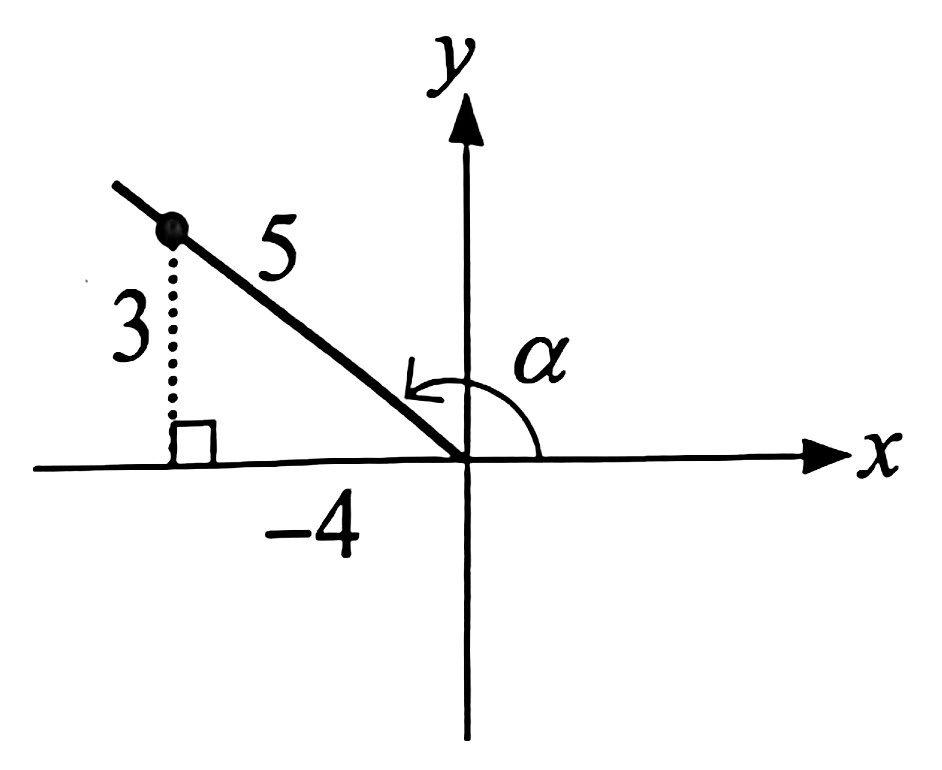
\includegraphics[width=0.25\textwidth]{assets/11-3.jpg}
		\end{center}
		\begin{center}
			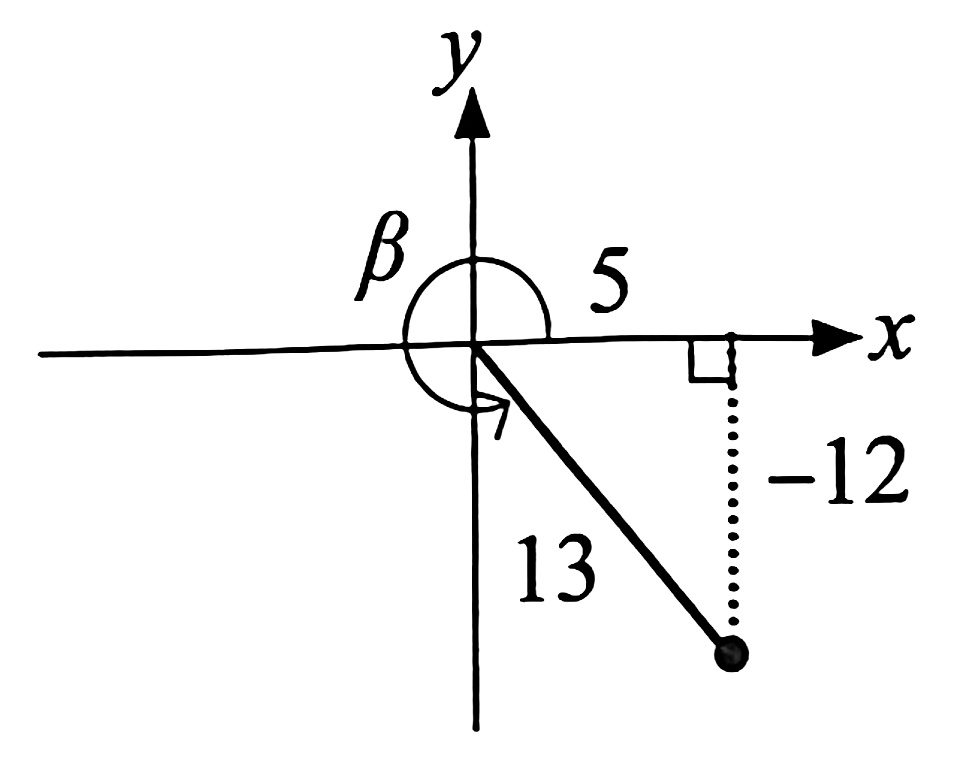
\includegraphics[width=0.25\textwidth]{assets/11-4.jpg}
		\end{center}
	\end{multicols}
\end{question}

\begin{question}
	Given that $\tan \alpha=\dfrac{1}{3}, \tan \beta=-2$, and $0^{\circ}<\alpha<90^{\circ}, 90^{\circ}<\beta<180^{\circ}$, find the value of $\alpha+\beta$.
	
	\sol{}
	
	\noindent From $\tan \alpha=\dfrac{1}{3}$, $\tan\beta = -2$, we have 
	
	\noindent $\begin{aligned} \tan (\alpha+\beta) & =\dfrac{\tan \alpha+\tan \beta}{1-\tan \alpha \tan \beta} \\ & =\dfrac{\dfrac{1}{3}+(-2)}{1-\left(\dfrac{1}{3}\right)(-2)} \\ & =-1\end{aligned}$
	
	\noindent Also, because $0^{\circ}<\alpha<90^{\circ}, 90^{\circ}<\beta<180^{\circ}$, therefore $90^{\circ}<\alpha+\beta<270^{\circ}$. In between $90^{\circ}$ and $270^{\circ}$, only the tangent value of $135^{\circ}$ is -1.
	
	\noindent $\therefore \alpha+\beta=135^{\circ}$
\end{question}

\practice{11.2c}
\begin{enumerate}
	\item Given that $\cos \alpha=\dfrac{3}{5}, \tan \beta=\dfrac{12}{5}$, where $\alpha$ is in the first quadrant and $\beta$ is in the third quadrant. Find the values of the following trigonometric functions:
	      \begin{tasks}[label=(\alph*)](2)
	      	\task $\cos (\alpha-\beta)$
	      	\task $\operatorname{cosec}(\alpha-\beta)$
	      \end{tasks}
	      
	\item Given that $\sin \alpha=\dfrac{5}{13}, \cos \beta=-\dfrac{4}{5}$, and both $\alpha$ and $\beta$ are angles in the same quadrant. Find the values of the following trigonometric functions:
	      \begin{tasks}[label=(\alph*)](2)
	      	\task $\sin (\alpha-\beta)$
	      	\task $\tan (\alpha+\beta)$
	      \end{tasks}
	      
	\item Given $\tan \alpha=2, \tan \beta=3$, and both $\alpha$ and $\beta$ are acute angles, prove that $\alpha+\beta=135^{\circ}$.
\end{enumerate}

\newpage
    
\begin{question}
	Given that line $l$ rotates counterclockwise from the $x$-axis by an angle $\theta$, then $\theta$ is called the inclination angle of line $l$. According to the definition, the relationship between the inclination angle $\theta$ of a line and its slope $m$ is $m=\tan \theta$. Now, consider two lines $l_1$ and $l_2$ with slopes $m_1$ and $m_2$ respectively. If the angle between line $l_1$ and line $l_2$ is $\alpha$, prove that $\tan \alpha=\dfrac{m_2-m_1}{1+m_2 m_1}$.
	
	\sol{}
	
	\begin{multicols}{2}
		\noindent Let the inclination angles of lines $l_1$ and $l_2$ be $\theta_1$ and $\theta_2$ respectively (as shown in the figure), then the slopes of lines $l_1$ and $l_2$ are $m_1=\tan \theta_1$ and $m_2=\tan \theta_2$ respectively.
		
		\noindent $\because$ $\alpha = \theta_2 - \theta_1$
		
		\noindent $\begin{aligned} \therefore \tan \alpha & =\tan \left(\theta_2-\theta_1\right) \\ & =\dfrac{\tan \theta_2-\tan \theta_1}{1+\tan \theta_2 \tan \theta_1} \\ & =\dfrac{m_2-m_1}{1+m_2 m_1}\end{aligned}$
		
		\begin{center}
			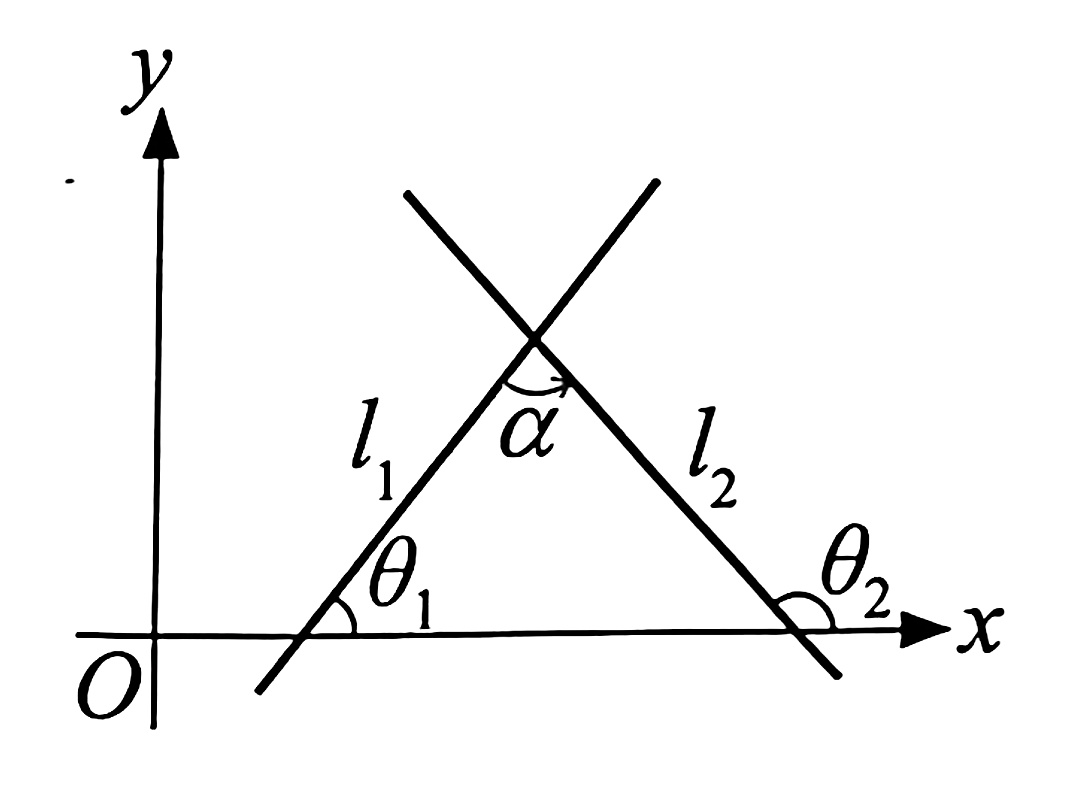
\includegraphics[width=0.3\textwidth]{assets/11-5.jpg}
		\end{center}
	\end{multicols}
\end{question}

\begin{think}
	    
	\noindent Under what circumstances does the formula $\tan \alpha=\dfrac{m_2-m_1}{1+m_2 m_1}$ not hold?
\end{think}

\practice{11.2d}

Given that the coordinates of the vertices of triangle $ABC$ are $A(1,5)$, $B(6,1)$, and $C(-2,-1)$. Find the interior angles of this triangle.

\newpage
We can utilize the sum and difference formulas for sine and cosine to transform expressions of the form $a \sin \theta+b \cos \theta$ into the form $R \sin (\theta \pm \alpha)$ or $R \cos (\theta \pm \alpha)$, where $R>0$ and $\alpha$ is an acute angle.

\begin{question}
	Express $\sin x+\sqrt{3} \cos x$ in the form $R \sin (x+\alpha)$, where $R>0$ and $\alpha$ is an acute angle.
	
	\sol{}
	
	\noindent Let $\begin{aligned}[t] \sin x+\sqrt{3} \cos x & =R \sin (x+\alpha) \\ \sin x+\sqrt{3} \cos x & =R \sin x \cos \alpha+R \cos x \sin \alpha \\ & =R \cos \alpha \sin x+R \sin \alpha \cos x\end{aligned}$
	
	\noindent Comparing the coefficients of $\sin x$ and $\cos x$ on both sides of the equation, we get 
	    
	$\begin{aligned}[t] R \cos \alpha & =1 &\cdots (1) \\ R \sin \alpha & =\sqrt{3} &\cdots (2)\end{aligned}$
	
	\noindent $(1)^2+(2)^2$ \ \ \ \ \ \ we get \ \ \ \ \ \ $
	\begin{aligned}[t]
		R^2\left(\cos ^2 \alpha+\sin ^2 \alpha\right) & =1^2+(\sqrt{3})^2   \\
		R                                             & =\sqrt{1+3}=2 (R>0) 
	\end{aligned}
	$
	
	\noindent $\dfrac{(2)}{(1)}$ \ \ \ \ \ \ \ \ \ \ \ \ \ \ \ \ \ \ \ \ we get \ \ \ \ \ \ $\begin{aligned}[t]
	\dfrac{\sin \alpha}{\cos \alpha} & =\dfrac{\sqrt{3}}{1} \\
	\tan \alpha & =\sqrt{3} \\
	\alpha & =\dfrac{\pi}{3}(\alpha \text { is acute angle })
	\end{aligned}
	$
	
	\noindent $\therefore \sin x+\sqrt{3} \cos x=2 \sin \left(x+\dfrac{\pi}{3}\right)$
\end{question}
\vspace{-1.5em}
\begin{center}
	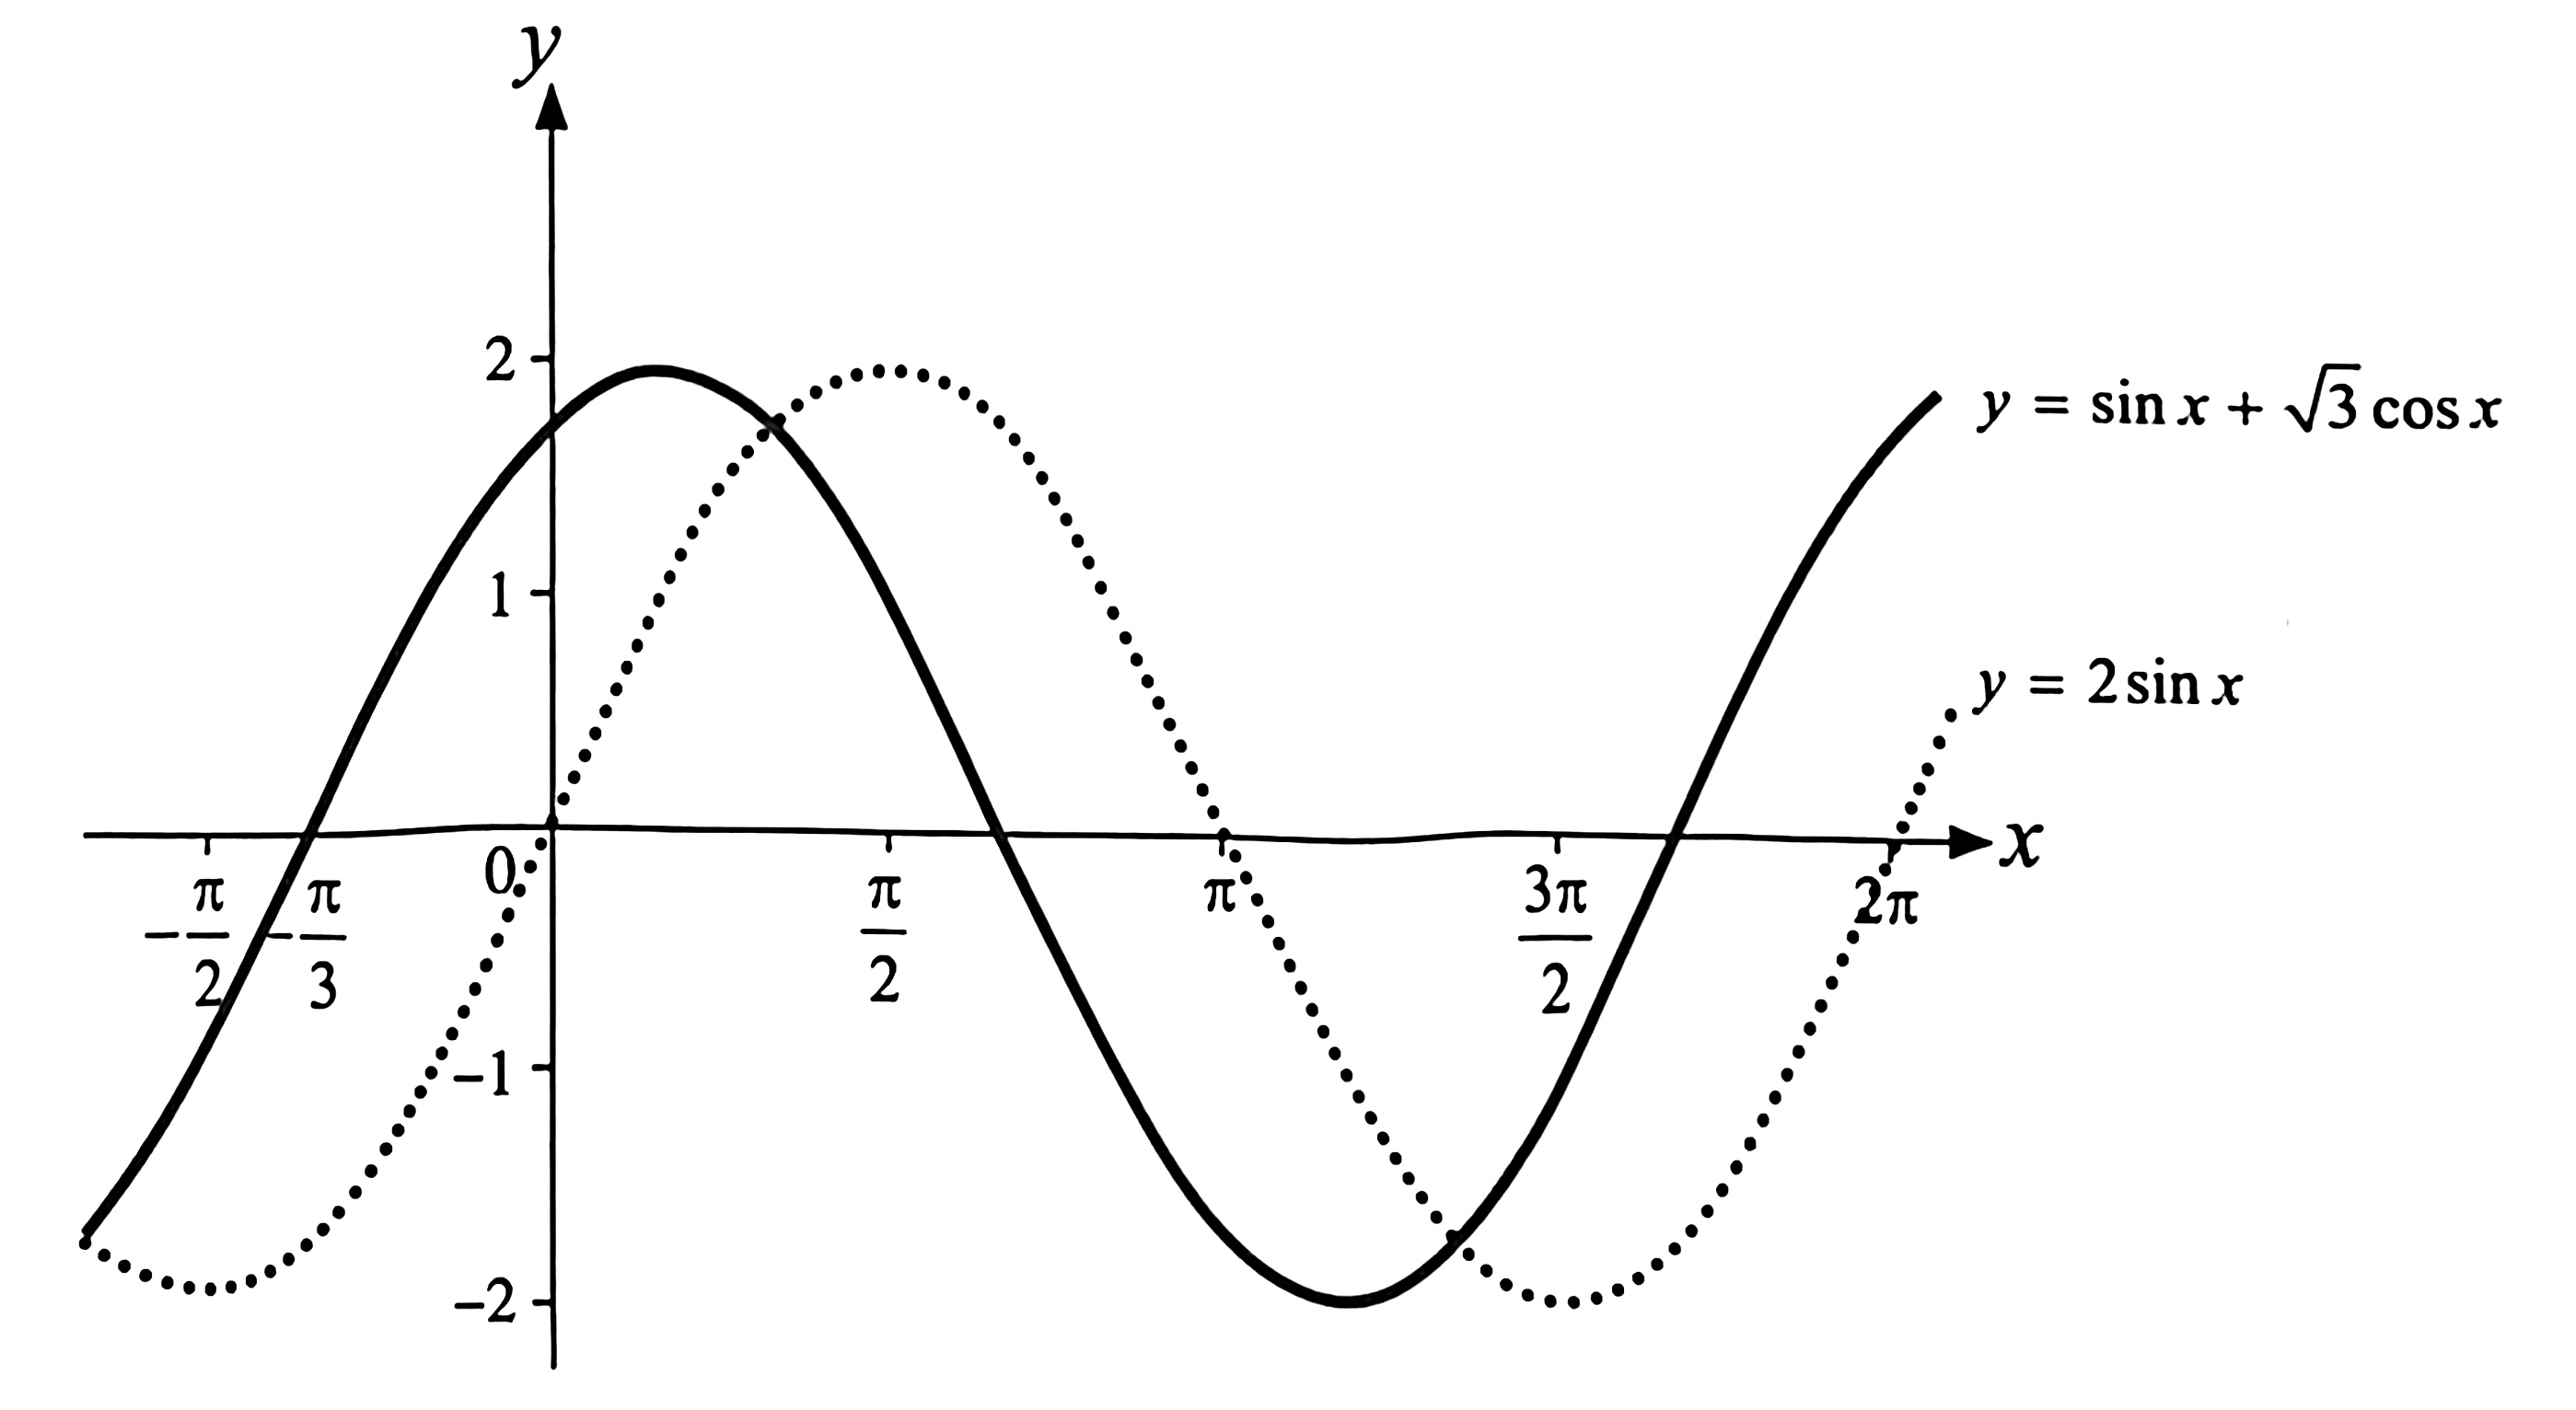
\includegraphics[width=0.55\textwidth]{assets/11-6.jpg}
\end{center}
\vspace{-2em}
From the figure above, we can also observe that the graph of $y=\sin x+\sqrt{3} \cos x$ is the curve of $y=2 \sin x$ shifted to the left along the $x$-axis by $\dfrac{\pi}{3}$, i.e. the graph of $y=2 \sin \left(x+\dfrac{\pi}{3}\right)$.

We can apply this transformation to determine the range of values of $\sin x+\sqrt{3} \cos x$.

$\begin{aligned} & \because-1 \leq \sin \left(x+\dfrac{\pi}{3}\right) \leq 1 \\ & -2 \leq 2 \sin \left(x+\dfrac{\pi}{3}\right) \leq 2 \\ & \therefore-2 \leq \sin x+\sqrt{3} \cos x \leq 2\end{aligned}$

\practice{11.2e}
\vspace{-1em}
\begin{enumerate}
	\item Express $f(x)=3 \cos x+\sqrt{3} \sin x$ in the form of $R \cos (x-\alpha)$, where $R>0$ and $\alpha$ is an acute angle. Hence, find the range of $f(x)$.
	\item Express $\cos \theta-\sqrt{3} \sin \theta$ in the form of $R \cos (\theta+\alpha)$. Hence, find the maximum and minimum values of $\cos \theta-\sqrt{3} \sin \theta$.
\end{enumerate}

\exercise{11.2}
\vspace{-1em}
\begin{enumerate}
	\item Without using a calculator, find the value of $\tan 32^{\circ} \tan 13^{\circ}+\tan 32^{\circ}+\tan 13^{\circ}$.
	\item Given $\sin \theta=\dfrac{15}{17}$ and $\dfrac{\pi}{2}<\theta<\pi$, without using a calculator, find the value of $\cos \left(\dfrac{\pi}{6}-\theta\right)$.
	\item Given $\sin \alpha=\dfrac{2}{3}$, $\cos \beta=-\dfrac{3}{4}$, and $\alpha$ and $\beta$ are angles in the same quadrant, without using a calculator, find the values of the following trigonometric functions:
	      \begin{tasks}[label=(\alph*)](4)
	      	\task $\sin (\alpha-\beta)$
	      	\task $\cos (\alpha-\beta)$
	      	\task $\tan (\alpha+\beta)$
	      	\task $\operatorname{cosec}(\alpha+\beta)$
	      \end{tasks}
	      
	\item Given $\sec A=\dfrac{17}{8}$, $\cot B=-\dfrac{3}{4}$, where $A$ is a quadrant I angle and $B$ is a quadrant II angle. Without using a computer, find the values of $\sec (A+B)$ and $\tan (A-B)$.
	\item Given the equations of the sides of a triangle as $4x-3y+9=0$, $12x-5y+15=0$, and $2x-y+1=0$. Find the interior angles of this triangle.
	              
\end{enumerate}
\vspace{-1em}

Prove the following identities (Question 6 to 16):
\vspace{-1em}
\begin{enumerate}[start=6]
	\item $\sin \left(\dfrac{5 \pi}{6}-A\right)+\sin \left(\dfrac{5 \pi}{6}+A\right)=\cos A$
	\item $\cos (A+B) \cos (A-B)=\cos ^2 A-\sin ^2 B$
	\item $\sin (A+B) \sin (A-B)=\sin ^2 A-\sin ^2 B$
	\item $\sin (A+B) \cos (A-B)=\sin A \cos A+\sin B \cos B$
	\item $\cos (A-B)-\sin (A+B)=(\cos A-\sin A)(\cos B-\sin B)$
	\item $\dfrac{\cos 2 A}{\sec A}-\dfrac{\sin 2 A}{\operatorname{cosec} A}=\cos 3 A$
	\item $\tan (A+B) \tan (A-B)=\dfrac{\tan ^2 A-\tan ^2 B}{1-\tan ^2 A \tan ^2 B}$
	\item $\dfrac{\tan A+\tan B}{\tan A-\tan B}=\dfrac{\sin (A+B)}{\sin (A-B)}$
	\item $\dfrac{\sin (A+B)}{\cos A \cos B}=\tan A+\tan B$
	\item $\dfrac{\tan (A-B)+\tan B}{1-\tan (A-B) \tan B}=\tan A$
	\item $1+\tan 2 A \tan A=\sec 2 A$
	\item Find the range of the following trigonometric functions:
	      \begin{enumerate}[label=(\alph*)]
	      	\item $f(x)=\sin x-\sqrt{3} \cos x$
	      	\item $f(x)=3 \sin x-4 \cos x$
	      \end{enumerate}
\end{enumerate}

\section{Trigonometric Functions of Double Angles}

From the trigonometric formulas for the sum of two angles, when $\beta=\alpha$, the corresponding double angle trigonometric formulas can be derived.
\begin{align*}
	\sin 2 \alpha & =\sin (\alpha+\alpha)                            \\
	              & =\sin \alpha \cos \alpha+\cos \alpha \sin \alpha \\
	              & =2 \sin \alpha \cos \alpha                       
\end{align*}
\begin{align*}
	\cos 2 \alpha & =\cos (\alpha+\alpha)                            \\
	              & =\cos \alpha \cos \alpha-\sin \alpha \sin \alpha \\
	              & =\cos ^2 \alpha-\sin ^2 \alpha                   \\
	              & =2 \cos ^2 \alpha-1                              \\
	              & =1-2 \sin ^2 \alpha                              
\end{align*}
\begin{align*}
	\tan 2 \alpha & =\tan (\alpha+\alpha)                                       \\
	              & =\dfrac{\tan \alpha+\tan \alpha}{1-\tan \alpha \tan \alpha} \\
	              & =\dfrac{2 \tan \alpha}{1-\tan ^2 \alpha}                    
\end{align*}

Listed below are the sine, cosine, and tangent formulas for double angles.
\begin{info}[Trigonometric Formulas of Double Angles]
	    
	$\begin{aligned} \sin 2 \alpha & =2 \sin \alpha \cos \alpha \\ \cos 2 \alpha & =\cos ^2 \alpha-\sin ^2 \alpha \\ & =2 \cos ^2 \alpha-1 \\ & =1-2 \sin ^2 \alpha \\ \tan 2 \alpha & =\dfrac{2 \tan \alpha}{1-\tan ^2 \alpha}\end{aligned}$
\end{info}

\begin{think}
	        
	\noindent Is there any other way to derive the tangent formula for double angles?
\end{think}

\newpage
\begin{question}
	Without using a calculator, find the values of the following expressions:
	\begin{tasks}[label=(\alph*)](2)
		\task $2 \cos ^2 15^{\circ}-1$
		\task $2 \sin \dfrac{\pi}{12} \cos \dfrac{\pi}{12}$
		\task $1-2 \sin ^2 75^{\circ}$
		\task $\dfrac{2 \tan 22.5^{\circ}}{1-\tan ^2 22.5^{\circ}}$
	\end{tasks}
	
	\sol{}
	\begin{enumerate}[label=(\alph*)]
		\item $\begin{aligned}[t]
		      2 \cos ^2 15^{\circ}-1 & =\cos 2\left(15^{\circ}\right) \\
		      & =\cos 30^{\circ} \\
		      & =\dfrac{\sqrt{3}}{2}
		\end{aligned}$
		\item $\begin{aligned}[t]
		      2 \sin \dfrac{\pi}{12} \cos \dfrac{\pi}{12} & =\sin \left(2 \times \dfrac{\pi}{12}\right) \\
		      & =\sin \dfrac{\pi}{6} \\
		      & =\dfrac{1}{2}
		\end{aligned}$
		\item $\begin{aligned}[t]
		      1-2 \sin ^2 75^{\circ} & =\cos 2\left(75^{\circ}\right) \\
		      & =\cos 150^{\circ} \\
		      & =-\dfrac{\sqrt{3}}{2}
		\end{aligned}$
		\item $\begin{aligned}[t]
		      \dfrac{2 \tan 22.5^{\circ}}{1-\tan ^2 22.5^{\circ}} & =\tan 2\left(22.5^{\circ}\right) \\
		      & =\tan 45^{\circ} \\
		      & =1
		\end{aligned}$
	\end{enumerate}
\end{question}

\begin{question}
	Without using a calculator, find the value of $\sin 22.5^{\circ}$.
	
	\sol{}
	    
	\noindent $\begin{aligned} \cos \left(2 \times 22.5^{\circ}\right) & =1-2 \sin ^2 22.5^{\circ} \\ \cos 45^{\circ} & =1-2 \sin ^2 22.5^{\circ} \\ \sin ^2 22.5^{\circ} & =\dfrac{1-\cos 45^{\circ}}{2} \\ & =\dfrac{2-\sqrt{2}}{4} \\ \sin 22.5^{\circ} & = \pm \dfrac{\sqrt{2-\sqrt{2}}}{2}\end{aligned}$
	
	\noindent $\because \sin 22.5^{\circ}>0, \therefore \sin 22.5^{\circ}=\dfrac{\sqrt{2-\sqrt{2}}}{2}$
\end{question}

\practice{11.3a}
\begin{enumerate}
	\item Without using a calculator, find the values of:
	      \begin{tasks}[label=(\alph*)](2)
	      	\task $2 \sin ^2 15^{\circ}-1$
	      	\task $2 \sin \dfrac{3 \pi}{8} \cos \dfrac{3 \pi}{8}$
	      	\task $\dfrac{2 \tan 165^{\circ}}{1-\tan ^2 165^{\circ}}$
	      	\task $\cos ^2 \dfrac{\pi}{8}-\sin ^2 \dfrac{\pi}{8}$
	      \end{tasks}
	\item Without using a calculator, find $\tan 22.5^{\circ}$.
	\item Given $\cos \theta=-\dfrac{4}{5}$ and $180^{\circ}<\theta<270^{\circ}$, find $\tan \dfrac{\theta}{2}$.
\end{enumerate}

\begin{question}
	Prove that $\dfrac{\sin 2 \alpha}{1-\cos 2 \alpha}=\cot \alpha 。$.
	
	\proof{}
	    
	\noindent $\begin{aligned} \dfrac{\sin 2 \alpha}{1-\cos 2 \alpha} & =\dfrac{2 \sin \alpha \cos \alpha}{1-\left(1-2 \sin ^2 \alpha\right)} \\ & =\dfrac{2 \sin \alpha \cos \alpha}{2 \sin ^2 \alpha} \\ & =\dfrac{\cos \alpha}{\sin \alpha} \\ & =\cot \alpha\end{aligned}$
\end{question}

\practice{11.3b}

Prove the following trigonometric identities:
\begin{enumerate}
	\item $\sin 2 x-2 \sin x+\cos x-1=(\cos x-1)(2 \sin x+1)$
	\item $\cot 2 x+\operatorname{cosec} 2 x=\cot x$
	\item $\cos 3 A=4 \cos ^3 A-3 \cos A$
\end{enumerate}

\newpage
\exercise{11.3}

\begin{enumerate}
	\item Given $\sin A=\dfrac{3}{5}$ and $\dfrac{\pi}{2}<A<\pi$, without using a calculator, find $\sin 2A$, $\cos 2A$, and $\tan 2A$.
	\item Given $\cos A=\dfrac{8}{17}$ and $270^{\circ}<A<360^{\circ}$, without using a calculator, find $\sin \dfrac{A}{2}$ and $\cos \dfrac{A}{2}$.
	\item Given $\cos \theta=\dfrac{24}{25}$ and $270^{\circ}<\theta<360^{\circ}$, without using a calculator, find the value of $\tan \dfrac{\theta}{2}$.
	\item Without using a calculator, prove:
	      \begin{tasks}[label=(\alph*)](2)
	      	\task $\sin \dfrac{\pi}{8}=\dfrac{1}{2} \sqrt{2-\sqrt{2}}$
	      	\task $\cos \dfrac{\pi}{8}=\dfrac{1}{2} \sqrt{2+\sqrt{2}}$
	      \end{tasks}
	\item Express $\sin 3x$ in terms of $\sin x$.
	\item Express $\tan 3x$ in terms of $\tan x$.
\end{enumerate}

\vspace{-1em}
Prove the following identities (Question 7 to 17):
\vspace{-1em}
\begin{enumerate}[start=7]
	\item $\cot \theta-\cot 2 \theta=\operatorname{cosec} 2 \theta$
	\item $\operatorname{cosec} \theta-\cot \theta=\tan \dfrac{\theta}{2}$
	\item $\dfrac{\sin \theta}{\cos \theta-\sin \theta}+\dfrac{\cos \theta}{\cos \theta+\sin \theta}=\sec 2 \theta$
	\item $\dfrac{1+\sin \theta}{1-\sin \theta}=\tan ^2\left(\dfrac{\pi}{4}+\dfrac{\theta}{2}\right)$
	\item $\cos 2 A=\dfrac{1-\tan ^2 A}{1+\tan ^2 A}$
	\item $1-\sin A=\left(\sin \dfrac{A}{2}-\cos \dfrac{A}{2}\right)^2$
	\item $\tan A-\cot A=-2 \cot 2 A$
	\item $\dfrac{\sin 3 A}{\sin A}-\dfrac{\cos 3 A}{\cos A}=2$
	\item $\dfrac{\cos A-\sin A}{\cos A+\sin A}=\sec 2 A-\tan 2 A$
	\item $\dfrac{\sin 2 A}{1+\cos 2 A} \cdot \dfrac{\cos A}{1+\cos A}=\tan \dfrac{A}{2}$
	\item $1+\sin A=2 \cos ^2\left(\dfrac{\pi}{4}-\dfrac{A}{2}\right)$
\end{enumerate}

\newpage
\section{Trigonometric Equations}

An equation involving trigonometry that contains unknown variables is called a \textbf{trigonometric equation}. For example: $2 \sin x-1=0$, $\cos \left(2 x+\dfrac{\pi}{3}\right)=-\dfrac{1}{2}$, $\sin x-\cos x=1$, etc.

All values of the unknown variables that satisfy the trigonometric equation are called solutions of the trigonometric equation. If none of the values of the variables satisfy the trigonometric equation, then the equation is said to have no solution.

Trigonometric equations come in many forms, and these equations can often be transformed into one or more basic trigonometric equations of the form $\sin x=a$, $\cos x=a$, $\tan x=a$. For such equations, we only need to find the solutions on one period interval to determine all the solutions of the trigonometric equation.

\subsection*{Conditional Solutions of Trigonometric Equations}

In the process of solving trigonometric equations, it is often necessary to specify the interval of the unknown variables. Therefore, the solutions obtained are conditional solutions of the trigonometric equation.

\begin{question}
	Solve the equation $2\sin x=1$ for $0^{\circ}\leq x<360^{\circ}$.
	
	\sol{}
	
	\begin{vwcol}[widths={0.6,0.4}, sep=0.8cm, justify=flush,rule=0pt]
		\noindent $\begin{aligned} 2\sin x & =1 \\ \sin x & =\dfrac{1}{2}\end{aligned}$
		
		\noindent Since $\sin x=\dfrac{1}{2}$ is positive, $x$ is an angle in the first quadrant or the second quadrant, as shown in the figure,
		
		\noindent $\therefore x=30^{\circ}, 150^{\circ}$
		
		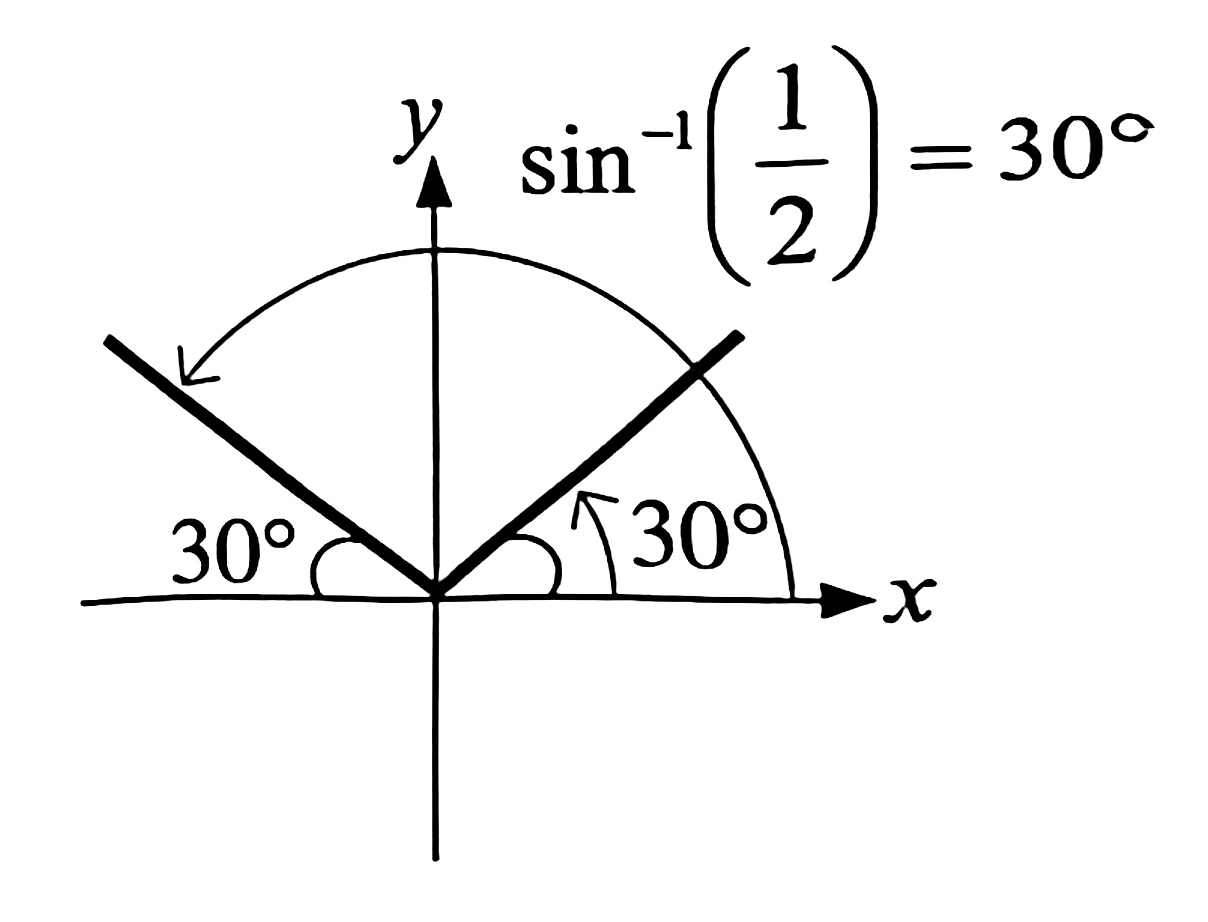
\includegraphics[width=0.3\textwidth]{assets/11-7.jpg}
	\end{vwcol}
\end{question}

\begin{question}
	Solve the equation $\tan 2 x=-\sqrt{3}$ for $0^{\circ} \leq x \leq 360^{\circ}$.
	
	\sol{}
	
	\begin{vwcol}[widths={0.6,0.4}, sep=0.8cm, justify=flush,rule=0pt]
		\noindent Given $0^{\circ} \leq x \leq 360^{\circ}$,
		    
		\noindent then $0^{\circ} \leq 2x \leq 720^{\circ}$.
		    
		\noindent Since $\tan 2x=-\sqrt{3}$ is negative, $2x$ is an angle in the second quadrant or the fourth quadrant, as shown in the figure,
		
		\noindent Therefore, $
		\begin{aligned}[t]
			2x & =120^{\circ}, 300^{\circ}, 120^{\circ}+360^{\circ}, 300^{\circ}+360^{\circ} \\
			x  & =60^{\circ}, 150^{\circ}, 240^{\circ}, 330^{\circ}                          
		\end{aligned}
		$
		
		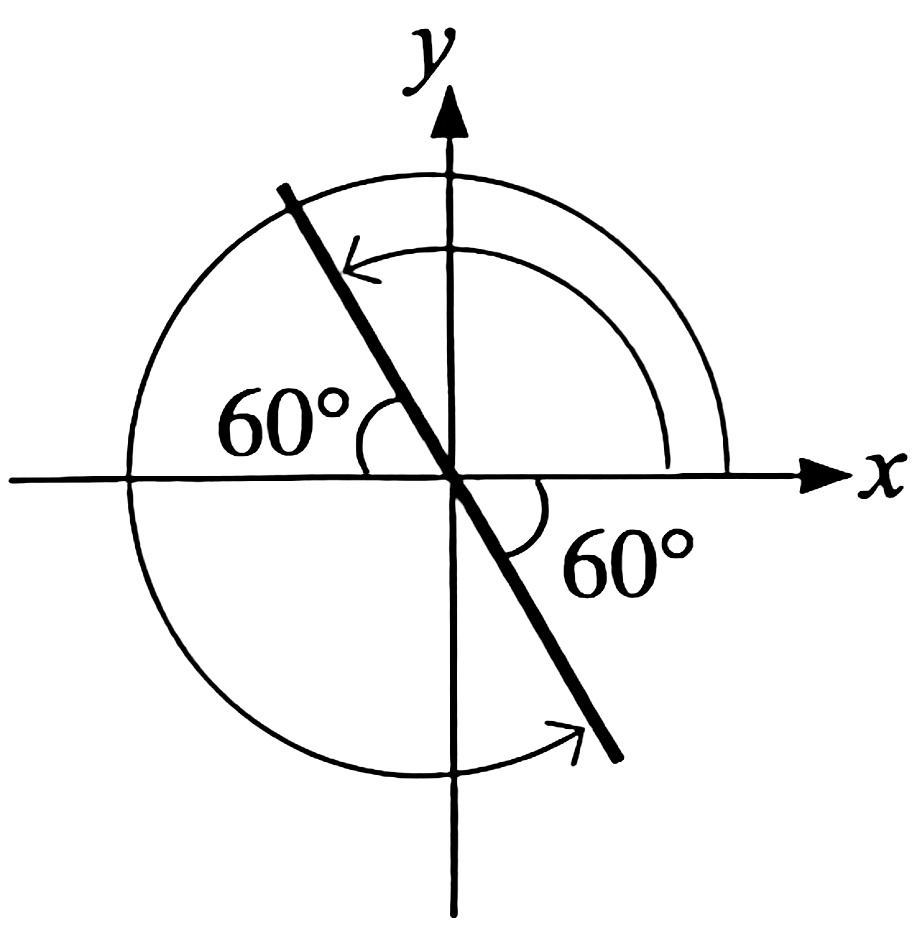
\includegraphics[width=0.22\textwidth]{assets/11-8.jpg}
		        
	\end{vwcol}
	\vspace{-2em}
	
\end{question}

\begin{question}
	Solve the equation $\cos \dfrac{x}{2}=-\dfrac{\sqrt{2}}{2},-180^{\circ} \leq x \leq 180^{\circ}$.
	
	\sol{}
	
	\noindent Given $-180^{\circ} \leq x \leq 180^{\circ}$,
	
	\vspace{-1em}
	\noindent then $-90^{\circ} \leq \dfrac{x}{2} \leq 90^{\circ}$,
	
	\vspace{-1em}
	\noindent so $\cos \dfrac{x}{2} \geq 0$, therefore, this equation has no solution.
\end{question}

\practice{11.4a}

Solve the following equations:
\begin{tasks}[label=(\alph*)](2)
	\task $\sin x=\dfrac{\sqrt{2}}{2},\ 0^{\circ} \leq x \leq 180^{\circ}$.
	\task $\cos x=\dfrac{\sqrt{3}}{2},\ -180^{\circ} \leq x \leq 180^{\circ}$.
	\task $\cot 3 x=\sqrt{3},\ 0^{\circ} \leq x \leq 360^{\circ}$.
	\task $\sqrt{3} \sin 2 x+\cos 2 x=0,\ 0^{\circ} \leq x \leq 360^{\circ}$.
\end{tasks}

\begin{question}
	Solve the equation $4 \sin ^2 x=3 \sin x$ for $0^{\circ} \leq x \leq 180^{\circ}$.
	
	\sol{}
	\begin{flalign*}
		4 \sin ^2 x&=3 \sin x &\\
		4 \sin ^2 x&-3 \sin x=0 \\
		\sin x(4 \sin x-3)&=0
	\end{flalign*}
	\vspace{-3em}
	\begin{flalign*}
		\sin x&=0 &&\text { or }& 4 \sin x-3&=0 &&&&&&&&&&&&&&&&&&\\
		x&=0^{\circ}, 180^{\circ}&&& \sin x&=\dfrac{3}{4}\\
		&&&&& x=48.59^{\circ}, 131.41^{\circ} 
	\end{flalign*}
	\noindent $\therefore x=0^{\circ}, 48.59^{\circ}, 131.41^{\circ}, 180^{\circ}$
\end{question}

\newpage
\begin{question}
	Solve the equation $2 \sin ^2 \theta+3 \sin \theta \cos \theta+\cos ^2 \theta=0$ for $0^{\circ} \leq \theta \leq 360^{\circ}$.
	
	\sol{}
	
	\noindent Since $\cos \theta \neq 0$, divide both sides of the equation by $\cos ^2 \theta$, we get
	\begin{flalign*}
		2 \tan ^2 \theta+3 \tan \theta+1 &=0 \\
		(2 \tan \theta+1)(\tan \theta+1)&=0 &
	\end{flalign*}
	\vspace{-3em}
	\begin{flalign*}
		2 \tan \theta+1&=0\ \ \ \ \ \ \ \ \ \ \ \ \ \ \ \ \ \  \text { or }&&& \tan \theta+1&=0 \\
		\tan \theta&=-\dfrac{1}{2} &&& \tan \theta&=-1 &&&&&&&&&&&&&&&&&&&&&&&&&&&&&&&&&&&&&&&&&&&&\\
		\theta&=153.43^{\circ}, 333.43^{\circ} &&& \theta&=135^{\circ}, 315^{\circ}&&
	\end{flalign*}
	\noindent $\therefore \theta=135^{\circ}, 153.43^{\circ}, 315^{\circ}, 333.43^{\circ}$
	
	\begin{think}
		        
		\noindent Why $\cos \theta \neq 0$?
	\end{think}
\end{question}

\begin{question}
	Solve the equation $2 \sin ^2 x+3 \cos x=0$ for $0 \leq x \leq 2 \pi$.
	
	\sol{}
	\begin{flalign*}
		2 \sin ^2 x+3 \cos x & =0 &\\
		2\left(1-\cos ^2 x\right)+3 \cos x & =0 \\
		2 \cos ^2 x-3 \cos x-2 & =0 \\
		(2 \cos x+1)(\cos x-2) & =0
	\end{flalign*}
	\vspace{-3em}
	\begin{flalign*}
		2 \cos x+1&=0 && \text { or } & \cos x-2&=0 &&&&&&&&&&&&&&&&&&&&&&&\\
		\cos x&=-\dfrac{1}{2} &&& \cos x&=2>1 \\
		x&=\dfrac{2 \pi}{3}, \dfrac{4 \pi}{3}  &&& \therefore \text{No}&\ {solution.}
	\end{flalign*}
	\noindent $\therefore x=\dfrac{2 \pi}{3}, \dfrac{4 \pi}{3}$
\end{question}

In the process of solving trigonometric equations, unless otherwise specified, angles are generally accurate to $0.01^{\circ}$ and radians are accurate to $0.0001$.

\practice{11.4b}

Solve the following equations:
\vspace{-1em}
\begin{enumerate}
	\item $3 \cos ^2 x-5 \cos x+2=0,\ 0^{\circ} \leq x \leq 360^{\circ}$.
	\item $6 \cos ^2 \theta+\cos \theta \sin \theta-\sin ^2 \theta=0,\ -180^{\circ} \leq \theta \leq 180^{\circ}$.
	\item $3 \sec ^2 \theta+4 \tan \theta=\tan \theta+3,\ 0 \leq \theta \leq 2 \pi$.
\end{enumerate}

\begin{question}
	Solve the equation $\cos 2 x+3 \cos x+2=0$ for $0 \leq x \leq 2 \pi$.
	
	\sol{}
	\begin{flalign*}
		\cos 2 x+3 \cos x+2&=0 &\\
		2 \cos ^2 x-1+3 \cos x+2&=0 \\
		2 \cos ^2 x+3 \cos x+1&=0 
	\end{flalign*}
	\vspace{-3em}
	\begin{flalign*}
		2 \cos x+1&=0 &&\text { or }& \cos x + 1&=0 &&&&&&&&&&&&&&&&&&&&&&&&&&&&&&&&&\\
		\cos x&=-\dfrac{1}{2} &&& \cos x&=-1\\
		x&=\dfrac{2 \pi}{3}, \dfrac{4 \pi}{3} &&& x&=\pi
	\end{flalign*}
	\noindent$\therefore x=\dfrac{2 \pi}{3}, \pi, \dfrac{4 \pi}{3}$ \\
\end{question}

\begin{question}
	Solve the equation $\sin 2 x-2 \sin x+\cos x-1=0$ for $-180^{\circ} \leq x \leq 180^{\circ}$ 。
	
	\sol{}
	\begin{flalign*}
		\sin 2 x-2 \sin x+\cos x-1 & =0 &\\
		2 \sin x \cos x-2 \sin x+\cos x-1 & =0 \\
		2 \sin x(\cos x-1)+\cos x-1 & =0 \\
		(\cos x-1)(2 \sin x+1) & =0
	\end{flalign*}
	\vspace{-3em}
	\begin{flalign*}
		\cos x-1&=0 && \text { or } & 2 \sin x+1&=0 &&&&&&&&&&&&&&&&&&&&&&&&&&&&&&\\
		\cos x&=1 &&& \sin x&=-\dfrac{1}{2} \\
		x&=0^{\circ} &&& x&=-150^{\circ},-30^{\circ}
	\end{flalign*}
	\noindent $\therefore x=-150^{\circ},-30^{\circ}, 0^{\circ}$
\end{question}

\practice{11.4c}
Solve the following equations:
\vspace{-1em}
\begin{enumerate}
	\item $\sin x \sin 2 x=\cos x,\ 0^{\circ} \leq x \leq 360^{\circ}$ 。
	\item $\cos 2 \theta+\sin \theta-1=0,\ 0 \leq \theta \leq 2 \pi$ 。
\end{enumerate}

\begin{question}
	Solve the equation $\sqrt{3} \cos x-\sin x=1$ for $0 \leq x \leq 2 \pi$ 。
	
	\sol{}
	    
	\noindent Let $\begin{aligned}[t] &\sqrt{3} \cos x-\sin x=R \cos (x+\alpha), R>0, x \text { is acute angle. } \\ &\sqrt{3} \cos x-\sin x=R \cos x \cos \alpha-R \sin x \sin \alpha\end{aligned}$
	
	\noindent Comparing the coefficients of both sides, we get $\begin{aligned}[t] R \cos \alpha & =\sqrt{3} & \cdots (1) \\ R \sin \alpha & =1 & \cdots (2) \end{aligned}$
	\begin{flalign*}
		&(1)^2+(2)^2 && \text { we get } & R^2(\cos ^2 \alpha+\sin ^2 \alpha) & =\left(\sqrt{3}\right)^2+1^2 &&&&&&&&&&&&&&&&\\
		&&&& R &= \sqrt{3 + 1} = 2\\
		& \dfrac{(2)}{(1)} && \text { we get } & \dfrac{\sin \alpha}{\cos \alpha} & =\dfrac{1}{\sqrt{3}}\\
		&&&& \tan \alpha & =\dfrac{1}{\sqrt{3}} \\
		&&&& \alpha & =\dfrac{\pi}{6}
	\end{flalign*}
	\noindent $
	\begin{aligned}
		\therefore2 \cos \left(x+\dfrac{\pi}{6}\right)=1 &                                        &  \\
		& \cos \left(x+\dfrac{\pi}{6}\right)=\dfrac{1}{2}
	\end{aligned}
	$
	
	\noindent From the condition $0 \leq x \leq 2 \pi$,
	
	\noindent we get
	$\begin{aligned}[t]
		  & \dfrac{\pi}{6} \leq x+\dfrac{\pi}{6} \leq \dfrac{13 \pi}{6} \\
		  & x+\dfrac{\pi}{6}=\dfrac{\pi}{3}, \quad 2 \pi-\dfrac{\pi}{3} \\
		  & \quad \therefore x=\dfrac{\pi}{6}, \dfrac{3 \pi}{2}         
	\end{aligned}
	$
\end{question}
\vspace{-2em}
\practice{11.4d}
Solve the following equations:
\vspace{-1em}
\begin{enumerate}
	\item $\cos x+\sqrt{3} \sin x=1,\ 0 \leq x \leq 2 \pi$.
	\item $5 \sin x-12 \cos x=13,\ 0^{\circ} \leq x \leq 360^{\circ}$.
\end{enumerate}

\exercise{11.4a}
\begin{enumerate}
	\item Solve the following trigonometric equations, where $0^{\circ} \leq x \leq 360^{\circ}$:
	      \begin{tasks}[label=(\alph*)](2)
	      	\task $4 \tan x+3 \sec x=0$
	      	\task $2 \sin ^2 x+5 \sin x \cos x+2 \cos ^2 x=0$
	      	\task $6 \sec ^2 x-\tan x=7$
	      	\task $\cos \left(x-30^{\circ}\right)=3 \sin \left(x-60^{\circ}\right)$
	      	\task $3 \cos 2 x+4 \cos x+3=0$
	      	\task $2 \sin 3 x+3 \cos 3 x=\sqrt{13}$
	      	\task $3 \cos x+4 \sin x=5$
	      \end{tasks}
	\item Solve the following trigonometric equations, where $-180^{\circ} \leq \theta \leq 180^{\circ}$L
	      \begin{tasks}[label=(\alph*)](2)
	      	\task $\cot \theta-2 \cos \theta=0$
	      	\task $7 \sin \theta+3 \cos \theta=0$
	      	\task $7 \operatorname{cosec}^2 \theta-13 \cot \theta=9$
	      	\task $2 \cos \theta \cot \theta=3$
	      	\task $3 \cos 2 \theta+8 \sin \theta+5=0$
	      	\task $2 \sin 2 \theta=3 \cos \theta$
	      	\task $5 \sin \theta+12 \cos \theta=7$
	      \end{tasks}
	\item Solve the following trigonometric equations, where $0 \leq x \leq 2 \pi$:
	      \begin{tasks}[label=(\alph*)](2)
	      	\task $2 \tan x \cos x+1=0$
	      	\task $4 \cos ^2 x+4 \sin x=1$
	      	\task $4 \sin 2 x=3 \operatorname{cosec} 2 x$
	      	\task $\tan x \tan 2 x=1$
	      	\task $\cos x-\sin x=\sqrt{2}$
	      	\task $\sqrt{3} \sin 2 x=1+\cos 2 x$
	      \end{tasks}
\end{enumerate}

Due to the periodic nature of trigonometric functions, a trigonometric equation generally has infinitely many solutions. We can represent the solutions of the equation using the method of a \textbf{general solution}.

\subsubsection*{(1) General Solution of $\mathbf{\text{sin } x=a}$}

\begin{question}
	Find the general solution of the equation $\sin x=\dfrac{1}{2}$.
	
	\sol{}
	
	\begin{vwcol}[widths={0.6,0.4}, sep=0.8cm, justify=flush,rule=0pt]
		\noindent First, find the solutions on one period interval of $\sin x=\dfrac{1}{2}$, as shown in the figure, 
		    
		\noindent we get $x_1=\dfrac{\pi}{6}, x_2=\pi-\dfrac{\pi}{6}$.
		
		\noindent Since the period of the sine function is $2\pi$, adding $2k\pi$ to each of $x_1$ and $x_2$ ($k$ is an integer), we obtain the general solution of the equation,
		
		\vspace{0.5em}
		\noindent $\begin{aligned} \therefore x & =2 k \pi+\dfrac{\pi}{6} &\cdots\ (1) \\ x & =2 k \pi+\pi-\dfrac{\pi}{6} \\ & =(2 k+1) \pi-\dfrac{\pi}{6}&\cdots\ (2)\end{aligned}$
		
		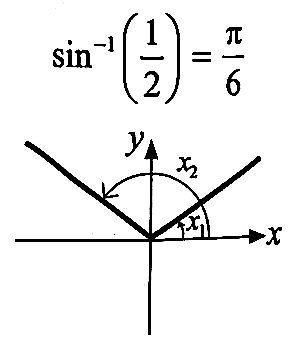
\includegraphics[width=0.2\textwidth]{assets/11-9.jpg}
	\end{vwcol}
\end{question}

In the above expression, $2k$ is even and $2k+1$ is odd. Let $n$ be an integer. When $n$ is even, $(-1)^n=+1$, and when $n$ is odd, $(-1)^n=-1$. Therefore, equations (1) and (2) can be combined as $x=n\pi+(-1)^n\dfrac{\pi}{6}, n \in \mathbb{Z}$.

\begin{question}
	Find the general solution of the equation $\sin x=-\dfrac{\sqrt{2}}{2}$.
	
	\sol{}
	
	\begin{vwcol}[widths={0.6,0.4}, sep=0.8cm, justify=flush,rule=0pt]
		\noindent First, find the solutions on one period interval of $\sin x=-\dfrac{\sqrt{2}}{2}$, as shown in the figure,
		        
		\noindent we get $x_1=-\dfrac{\pi}{4}, x_2=-\pi-\left(-\dfrac{\pi}{4}\right)$.
		
		\noindent Since the period of the sine function is $2\pi$, adding $2k\pi$ to each of $x_1$ and $x_2$ ($k$ is an integer), we obtain the general solution of the equation,
		
		\vspace{1em}
		\noindent $\begin{aligned} \therefore x & =2 k \pi+\left(-\dfrac{\pi}{4}\right)  &\cdots\ (1)\\ x & =2 k \pi-\pi-\left(-\dfrac{\pi}{4}\right) \\ & =(2 k-1) \pi-\left(-\dfrac{\pi}{4}\right) &\cdots\ (2)\end{aligned}$
		
		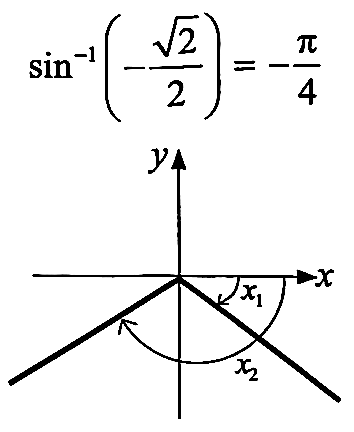
\includegraphics[width=0.2\textwidth]{assets/11-10.jpg}
	\end{vwcol}
	\vspace{-1em}
	\noindent Equations (1) and (2) can be combined as $x=n\pi+(-1)^n\left(-\dfrac{\pi}{4}\right), n \in \mathbb{Z}$.
\end{question}

\begin{question}
	Find the general solution of the equation $\sin ^3 x-\sin x=0$.
	
	\sol{}
	\vspace{-1em}
	\begin{multicols}{2}
		\noindent $\begin{aligned} \sin ^3 x-\sin x & =0 \\ \sin x(\sin x-1)(\sin x+1) & =0\end{aligned}$
		    
		\noindent From the graph of the sine function,
		
		\vspace{-1em}
		\noindent the general solution of $\sin x=0$ is $x=n\pi$,
		
		\vspace{-1em}
		\noindent the general solution of $\sin x=1$ is $x=2n\pi+\dfrac{\pi}{2}$,
		
		\vspace{-1em}
		\noindent the general solution of $\sin x=-1$ is $x=2n\pi-\dfrac{\pi}{2}$,
		
		\vspace{-1em}
		\noindent $\therefore x=\dfrac{n\pi}{2}, n \in \mathbb{Z}$.
		\vspace{5em}
		
		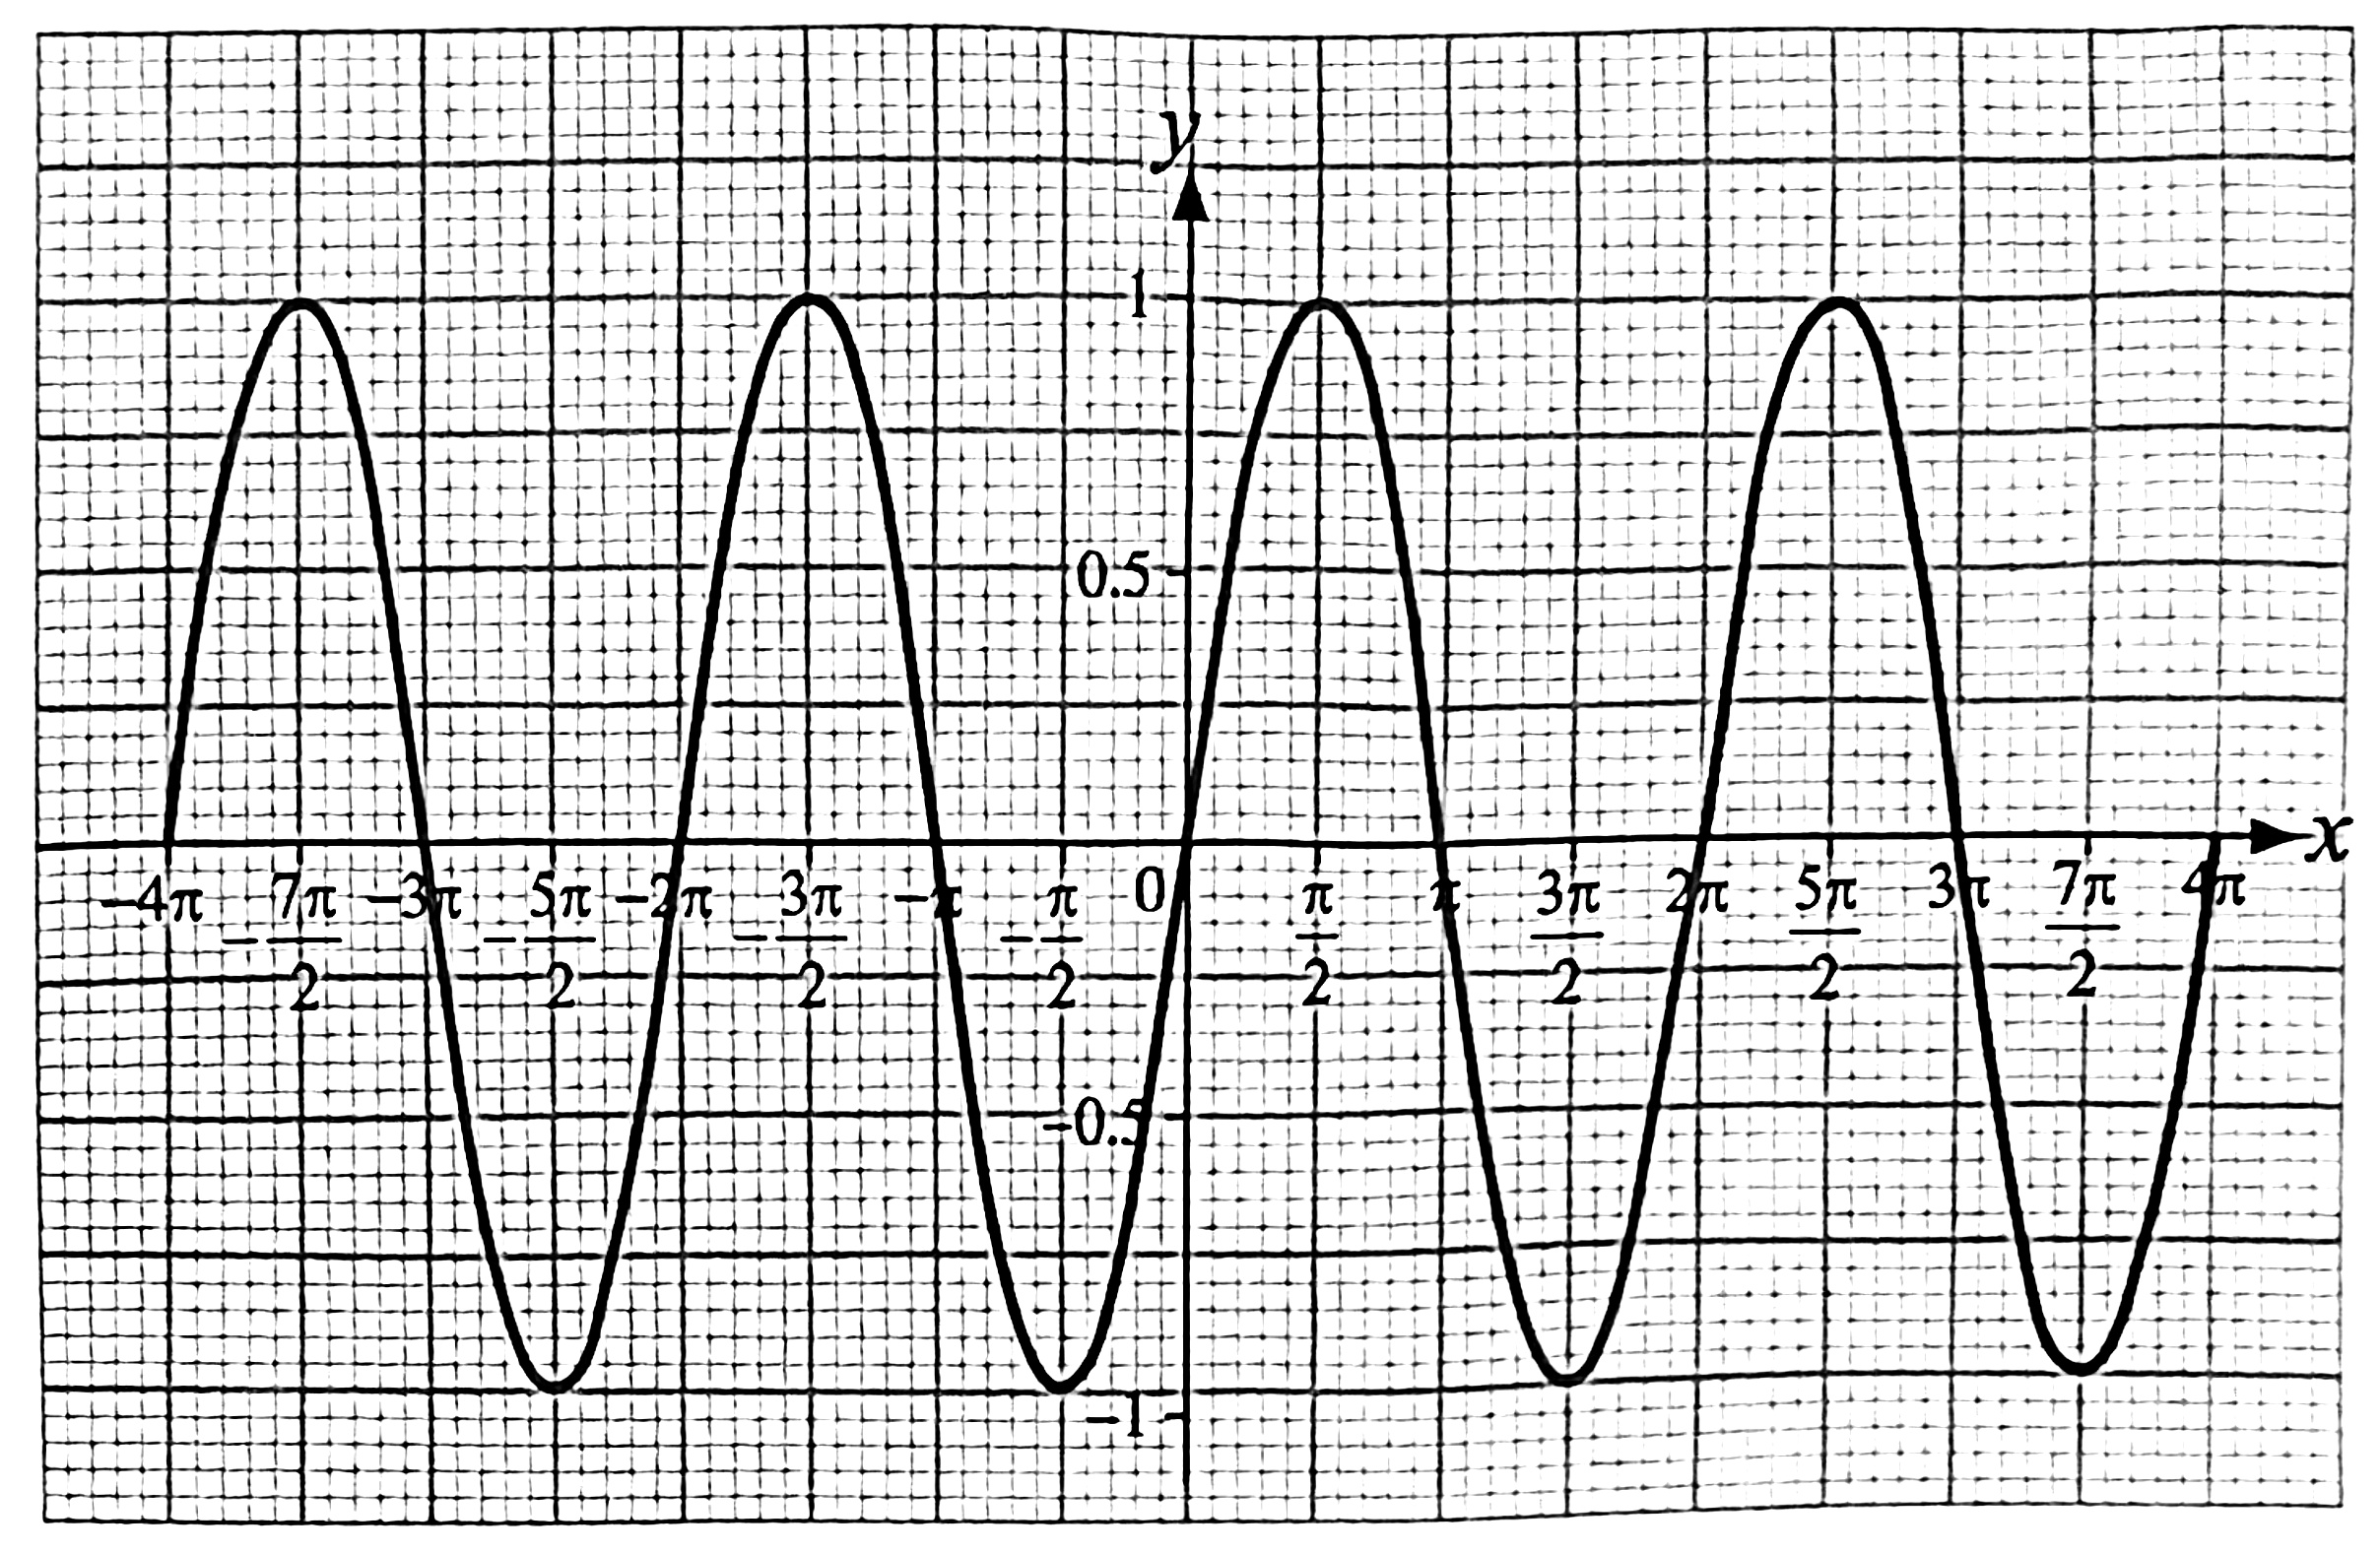
\includegraphics[width=0.4\textwidth]{assets/11-11.jpg}
	\end{multicols}
\end{question}

\practice{11.4e}
Find the general solution of the equation $2 \sin ^2 x-\sin x-1=0$.

\subsubsection*{(2) General Solution of $\mathbf{\text{cos } x=a}$}

\begin{question}
	Find the general solution of the equation $\cos x=\dfrac{\sqrt{2}}{2}$.
	
	\sol{}
	    
	\begin{vwcol}[widths={0.6,0.4}, sep=0.8cm, justify=flush,rule=0pt]
		\noindent First, find the solutions on one period interval of $\cos x=\dfrac{\sqrt{2}}{2}$, as shown in the figure,
		
		\noindent we get $x_1=\dfrac{\pi}{4}, x_2=-\dfrac{\pi}{4}$.
		
		\noindent Since the period of the cosine function is $2\pi$, adding $2k\pi$ to each of $x_1$ and $x_2$ ($k$ is an integer), we obtain the general solutions of the equation,
		
		\vspace{1em}
		\noindent $
		\begin{aligned}
			\therefore x & =2k\pi+\dfrac{\pi}{4} & \cdots\ (1) \\
			x            & =2k\pi-\dfrac{\pi}{4} & \cdots\ (2) 
		\end{aligned}
		$
		
		\noindent Equations (1) and (2) can be combined as $x=2n\pi\pm\dfrac{\pi}{4}, n \in \mathbb{Z}$.
		\vspace{2em}
		
		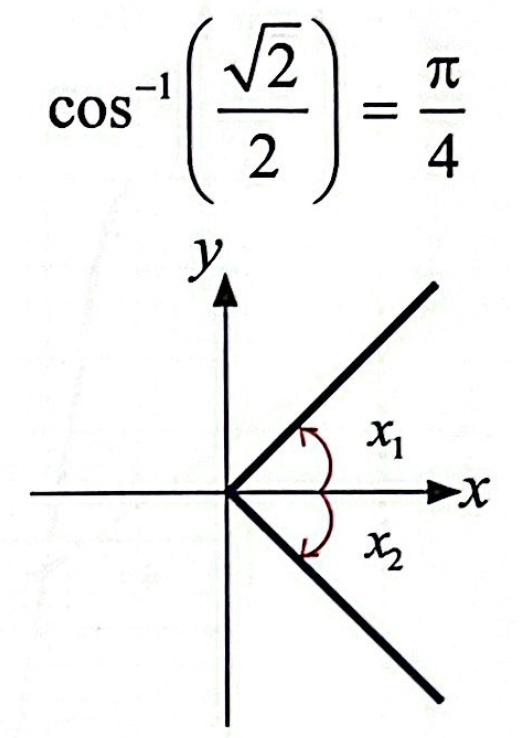
\includegraphics[width=0.2\textwidth]{assets/11-12.jpg}
	\end{vwcol}
	\vspace{-0.2em}
\end{question}

\begin{question}
	Find the general solution of the equation $\cos x=-\dfrac{\sqrt{3}}{2}$.
	
	\sol{}
	\begin{vwcol}[widths={0.6,0.4}, sep=0.8cm, justify=flush,rule=0pt]
		\noindent First, find the solutions on one period interval of $\cos x=-\dfrac{\sqrt{3}}{2}$, as shown in the figure,
		
		\noindent we get $x_1=\dfrac{5\pi}{6}, x_2=-\dfrac{5\pi}{6}$.
		
		\noindent Since the period of the cosine function is $2\pi$, adding $2k\pi$ to each of $x_1$ and $x_2$ ($k$ is an integer), we obtain the general solutions of the equation,
		        
		\vspace{1em}
		\noindent $
		\begin{aligned}
			\therefore x & =2k\pi+\dfrac{5\pi}{6} \\
			x            & =2k\pi-\dfrac{5\pi}{6} 
		\end{aligned}
		$
		
		\noindent Equations (1) and (2) can be combined as $x=2n\pi\pm\dfrac{5\pi}{6}, n \in \mathbb{Z}$.
		\vspace{2em}
		
		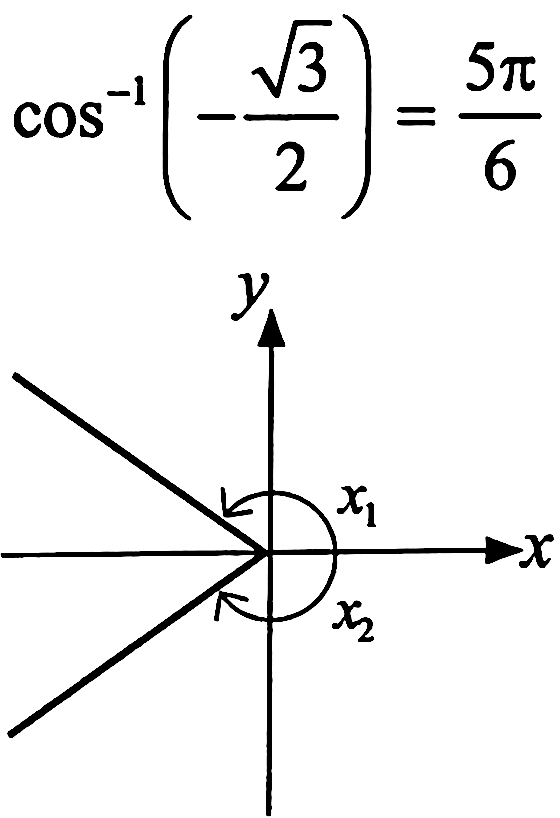
\includegraphics[width=0.2\textwidth]{assets/11-13.jpg}
	\end{vwcol}
	\vspace{-1em}
\end{question}
\newpage
\begin{question}
	Find the general solution of the equation $\cos ^3 x-\cos x=0$.
	
	\sol{}
	\begin{multicols}{2}
		\noindent $\begin{aligned} & \cos ^3 x-\cos x=0 \\ & \cos x(\cos x-1)(\cos x+1)=0\end{aligned}$
		   
		\noindent From the graph of the cosine function,
		
		\vspace{-1em}
		\noindent the general solution of $\cos x=0$ is $x=(2n+1)\dfrac{\pi}{2}$,
		    
		\vspace{-1em}
		\noindent the general solution of $\cos x=1$ is $x=2n\pi$,
		
		\vspace{-1em}
		\noindent the general solution of $\cos x=-1$ is $x=(2n+1)\pi$,
		
		\vspace{-1em}
		\noindent $\therefore x=\dfrac{n\pi}{2}, n \in \mathbb{Z}$.
		\columnbreak
		
		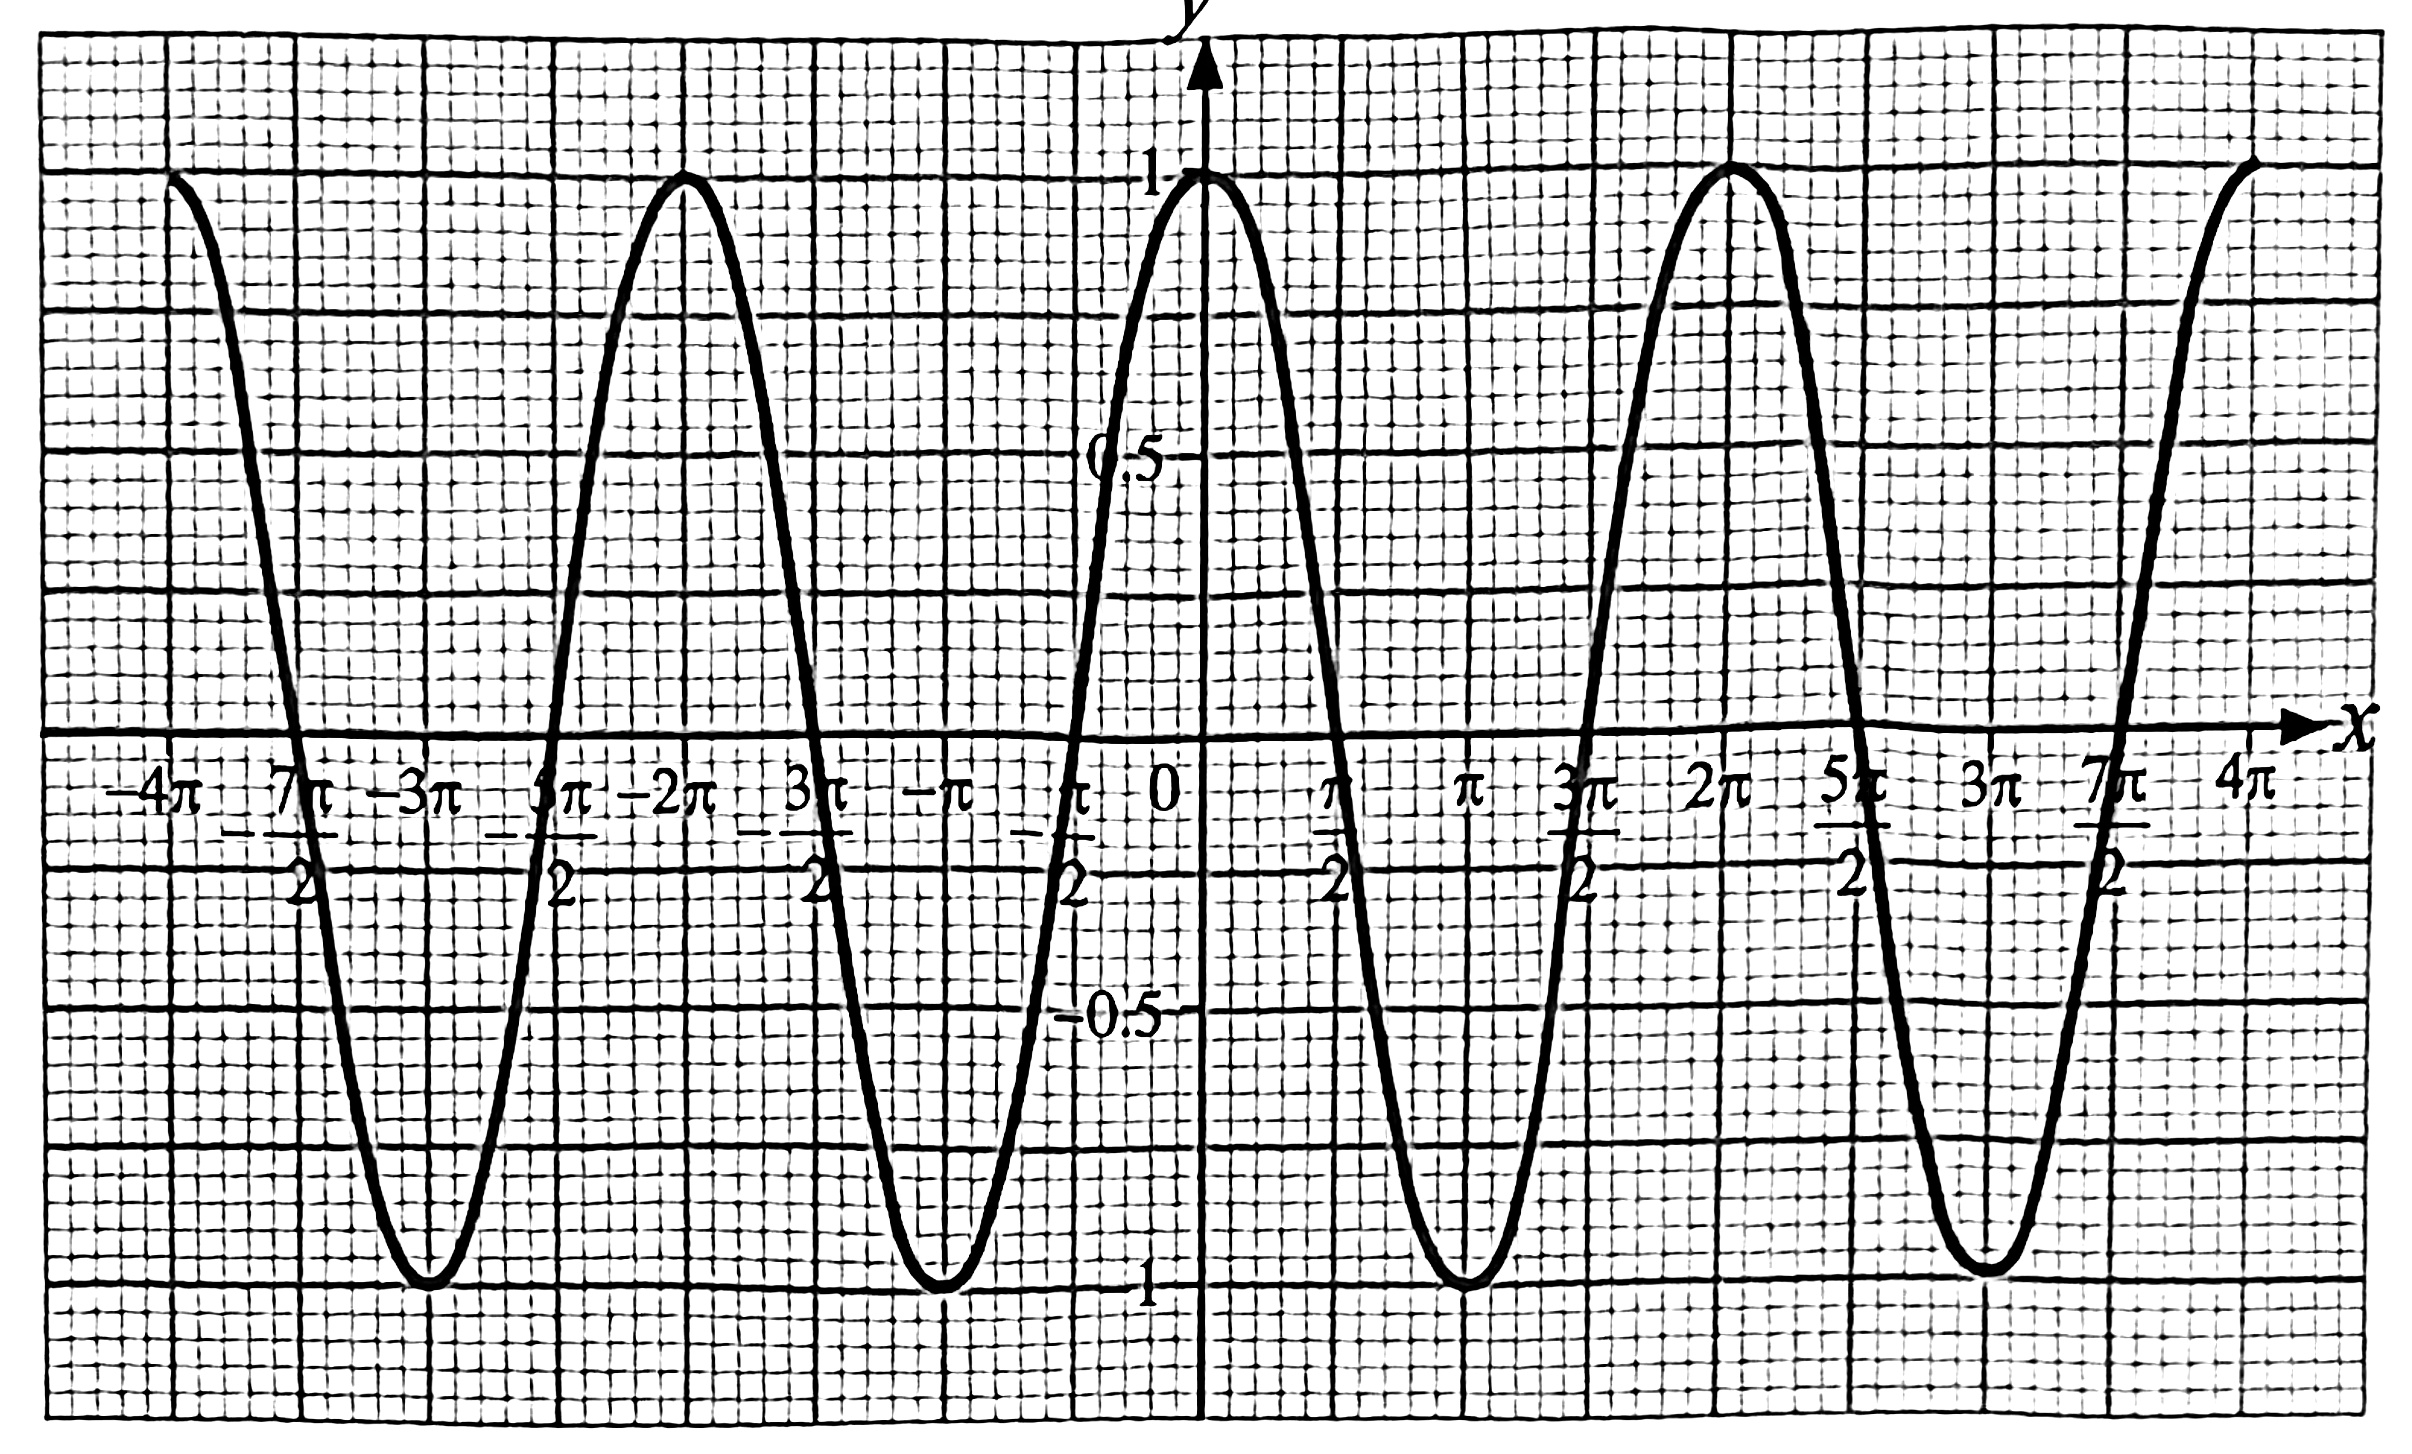
\includegraphics[width=0.4\textwidth]{assets/11-14.jpg}
	\end{multicols}
\end{question}

\practice{11.4f} 

Find the general solution of the equation $2 \cos ^2 x+\cos x-1=0$.

\subsubsection*{(3) General Solution of $\mathbf{\text{tan } x=a}$}

\begin{question}
	Find the general solution of the equation $\tan x=\sqrt{3}$.
	
	\sol{}
	\begin{vwcol}[widths={0.6,0.4}, sep=0.8cm, justify=flush,rule=0pt]
		\noindent First, ind the solutions of the equation $\tan x = \sqrt{3}$ within one period, as shown in the diagram,
		
		\noindent we get $x_1=\dfrac{\pi}{3}, x_2=\pi+\dfrac{\pi}{3}$.
		
		\noindent Since the period of the tangent function is $\pi$, adding $k\pi$ to each of $x_1$ and $x_2$ ($k$ is an integer), we obtain the general solutions of the equation,
		
		\vspace{1em}
		\noindent $
		\begin{aligned}
			\therefore x & =k\pi+\dfrac{\pi}{3}     & \cdots\ (1) \\
			x & =k\pi+\pi+\dfrac{\pi}{3} \\
			             & =(k+1)\pi+\dfrac{\pi}{3} & \cdots\ (2) 
		\end{aligned}
		$
		
		\noindent Equations (1) and (2) can be combined as $x=n\pi+\dfrac{\pi}{3}, n \in \mathbb{Z}$.
		\vspace{2em}
		
		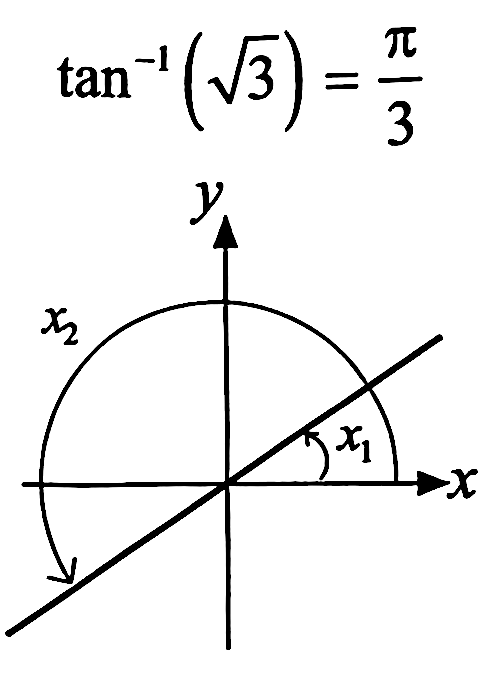
\includegraphics[width=0.2\textwidth]{assets/11-15.jpg}
	\end{vwcol}
\end{question}

\begin{question}
	Find the general solution of the equation $\tan x=-\dfrac{1}{\sqrt{3}}$.
	
	\sol{}
	\begin{vwcol}[widths={0.6,0.4}, sep=0.8cm, justify=flush,rule=0pt]
		\noindent First, find the solutions of the equation $\tan x=-\dfrac{1}{\sqrt{3}}$ within one period, as shown in the diagram,
		
		\noindent we get $x_1=-\dfrac{\pi}{6}, x_2=-\pi-\dfrac{\pi}{6}$.
		
		\noindent Since the period of the tangent function is $\pi$, adding $k\pi$ to each of $x_1$ and $x_2$ ($k$ is an integer), we obtain the general solutions of the equation,
		
		\vspace{1em}
		\noindent $
		\begin{aligned}
			\therefore x & =k\pi-\dfrac{\pi}{6}     & \cdots\ (1) \\
			x & =k\pi-\pi-\dfrac{\pi}{6} \\
			             & =(k-1)\pi-\dfrac{\pi}{6} & \cdots\ (2) 
		\end{aligned}
		$
		
		\noindent Equations (1) and (2) can be combined as $x=n\pi-\dfrac{\pi}{6}, n \in \mathbb{Z}$.
		\vspace{4em}
		
		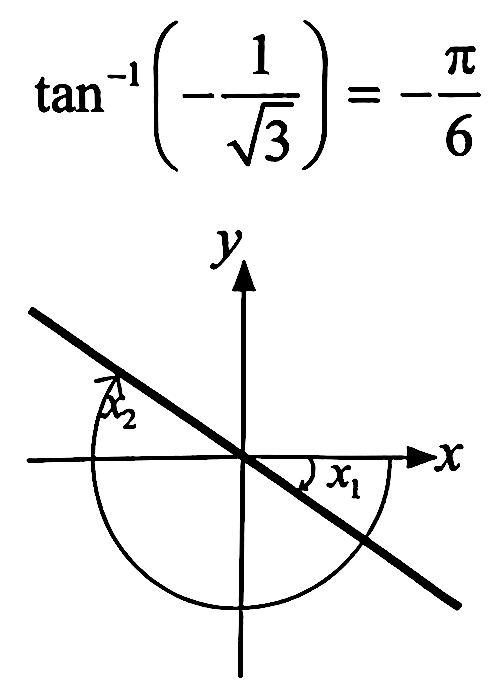
\includegraphics[width=0.22\textwidth]{assets/11-16.jpg}
	\end{vwcol}
	\vspace{-1em}
\end{question}

\practice{11.4g}

Find the general solution for the equation $3\sec^2\theta + 5\tan\theta = 2$.

\exercise{11.4b}

Find the general solution of the following equations:
\begin{enumerate}
	\item $\sin ^2 \theta-\cos ^2 \theta=\cos \theta$
	\item $\tan x=3 \cos x \operatorname{cosec} x$
	\item $\dfrac{1+\tan ^2 x}{1-\tan ^2 x}=2$
	\item $\cos 2 \theta-\cos \theta=0$
	\item $3 \sin \theta+\cos 2 \theta=2$
	\item $\sin x \cos x=\dfrac{\sqrt{2}}{4}$
	\item $2 \sin ^2 x+7 \sin x \cos x+6 \cos ^2 x=0$
	\item $\sin 2 x=\cos 2 x-\cos ^2 x+1$
	\item $\sqrt{3} \cos x-\sin x=\sqrt{3}$
	\item $2 \cos 2 x-2 \sin 2 x=\sqrt{6}$
\end{enumerate}

\subsubsection*{Graphical Method of Solving Trigonometric Equations}

An equation $f(x) = 0$ can be rewritten as two functions $y = g(x)$ and $y = h(x)$ such that $f(x) = g(x) - h(x) = 0$. The solutions to the equation $f(x) = 0$ are the values of the independent variable $x$ for which the values of the functions $y = g(x)$ and $y = h(x)$ are equal. Therefore, the $x$-coordinates of the intersection points of the graphs of the functions $y = g(x)$ and $y = h(x)$ in the Cartesian coordinate system are the solutions to the original equation $f(x) = 0$.

\begin{question}
	Solve the trigonometric equation $2 \sin \left(2 x+\dfrac{\pi}{3}\right)-4 \cos 2 x+1=0$ graphically, where $0 \leq x \leq \pi$.
	
	\sol{}
	
	\noindent Convert the equation into $2 \sin \left(2 x+\dfrac{\pi}{3}\right)=4 \cos 2 x-1$
	
	\noindent Let $g(x)=2 \sin \left(2 x+\dfrac{\pi}{3}\right), h(x)=4 \cos 2 x-1$
	
	\noindent We can construct the graphs of $\sin x$ and $\cos x$ and then apply transformations such as stretching, shrinking, and shifting to obtain the graphs of $g(x)$ and $h(x)$. The solutions to the equation are the $x$-coordinates of the intersection points of the graphs of $g(x)$ and $h(x)$ within the specified interval $0\leq x\leq \pi$.
	\begin{center}
		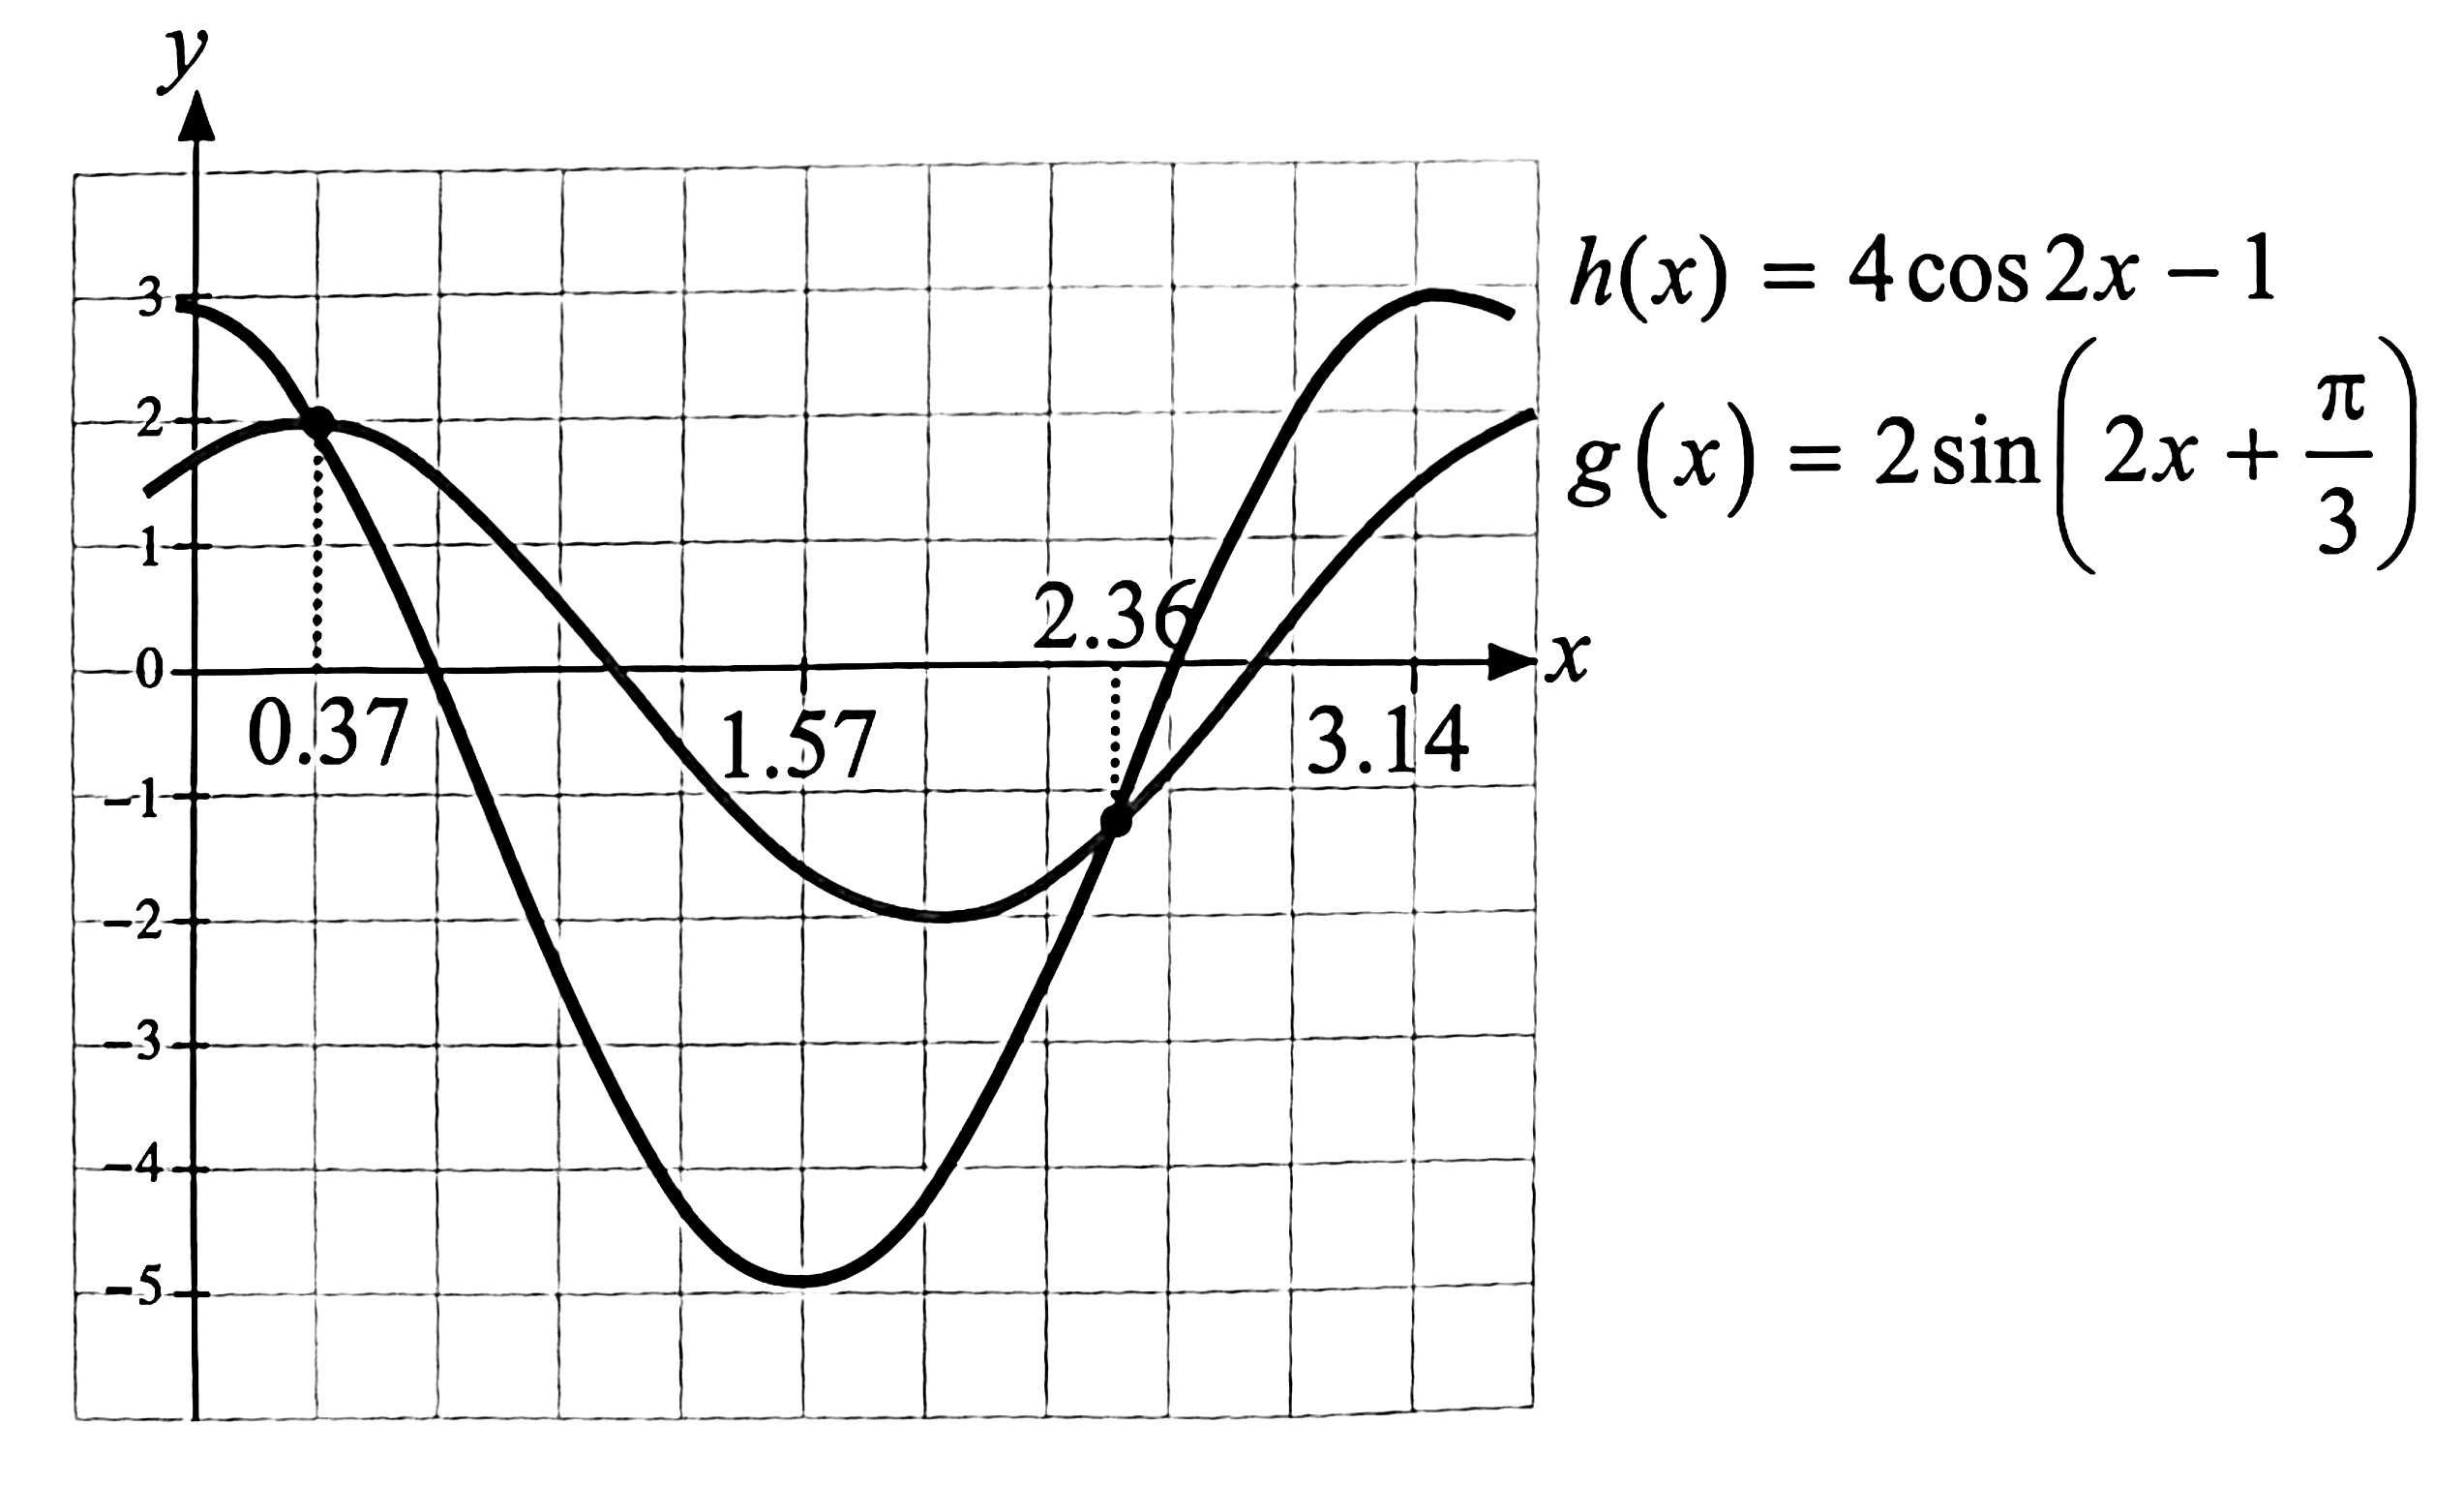
\includegraphics[width=0.55\textwidth]{assets/11-17.jpg}
	\end{center}
	\vspace{-1em}
	Based on the graph provided, the approximate values of x are 0.37 and 2.36.
\end{question}

\begin{question}
	Use the graphical method to find the number of solutions of the equation $2\cos x = x + 1$ in the interval $0 \leq x \leq 2\pi$.
	
	\sol{}
	
	\noindent Let $g(x) = 2\cos x, h(x) = x + 1$
	\vspace{-2em}
	\begin{center}
		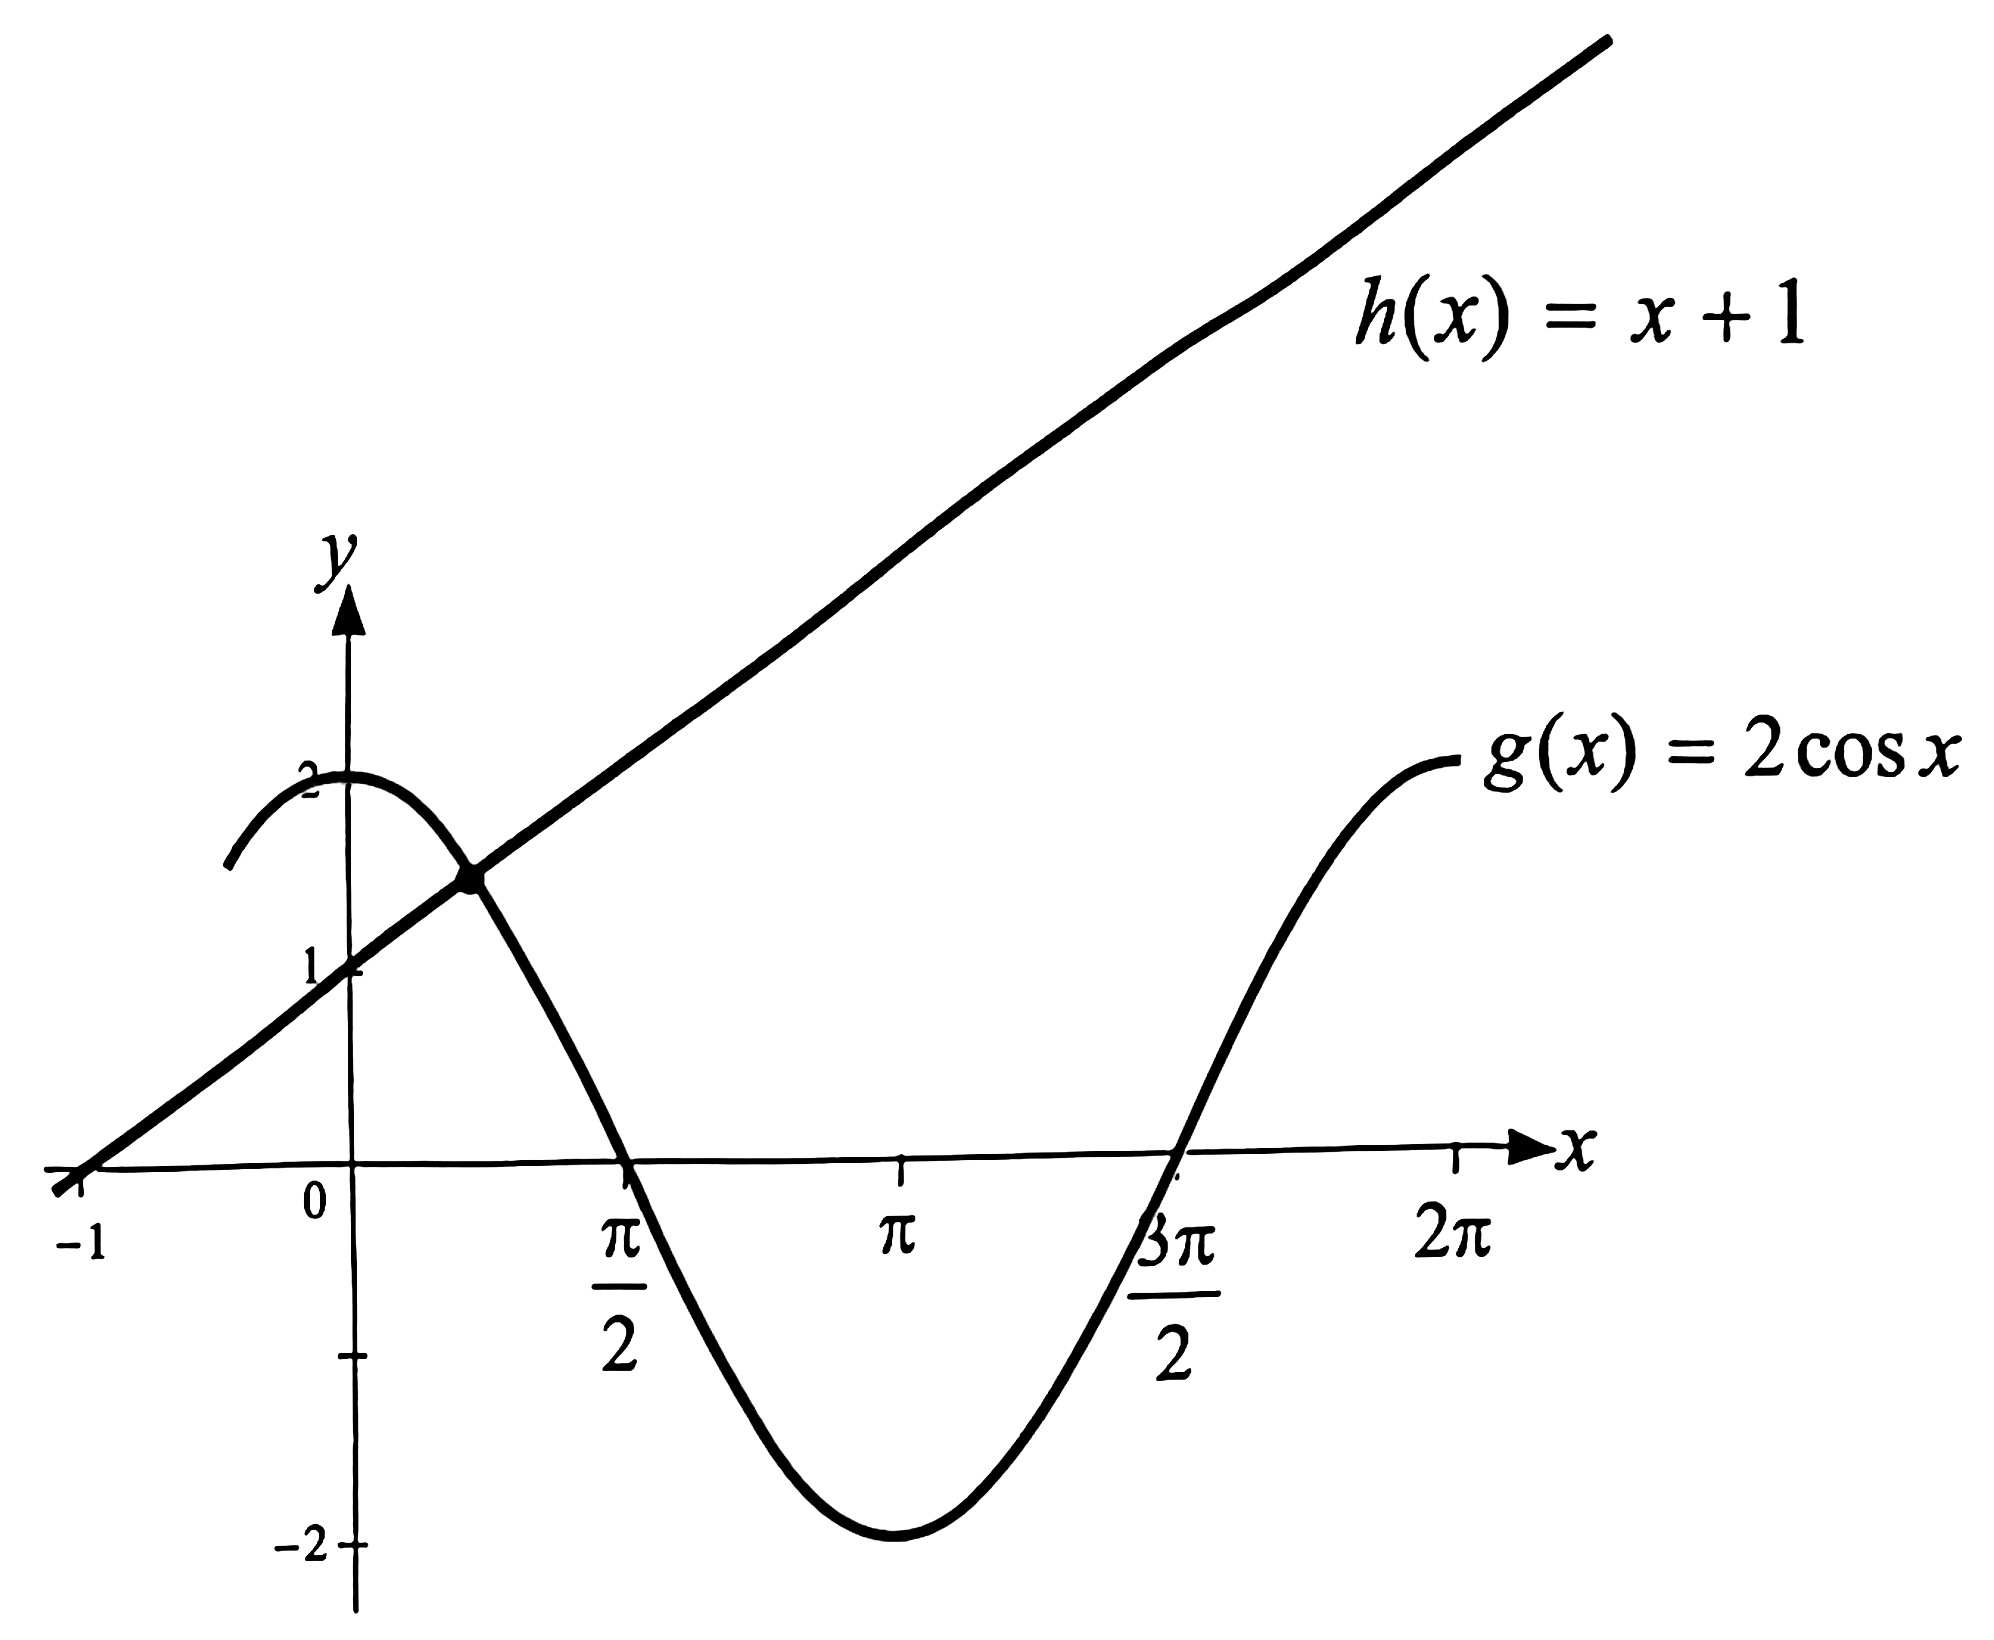
\includegraphics[width=0.5\textwidth]{assets/11-18.jpg}
	\end{center}
	\vspace{-2em}
	As shown in the figure above, since there is only one point of intersection of the graphs of the functions $y = g(x)$ and $y = h(x)$ in the interval $0 \leq x \leq 2\pi$, the equation $2\cos x = x + 1$ has only one solution in the interval $0 \leq x \leq 2\pi$.
\end{question}

\exercise{11.4c}
\begin{enumerate}
	\item Solve the equation $\sin x - \sin \dfrac{x}{2} = 0$ in the interval $0 \leq x \leq 2 \pi$ by graphing.
	          
	\item Find the number of solutions to the following equations in the given intervals by graphing:
	          
	      \begin{tasks}
	      	\task $\sin x + 2 \cos x = 1.5,\ 0 \leq x \leq \pi$
	      	\task $2 \cos x + \dfrac{x}{2} - 1 = 0,\ 0 \leq x \leq 2 \pi$
	      	\task $\sin x - x + 1 = 0,\ 0 \leq x \leq 2 \pi$
	      	\task $3 \sin x - \dfrac{x}{\pi} - 1 = 0,\ 0 \leq x \leq \pi$
	      \end{tasks}
\end{enumerate}

\newpage
\revision{11}
\begin{enumerate}
	\item Given $\sin \alpha = -\dfrac{3}{5}$ and $\cos \beta = -\dfrac{5}{13}$, and both $\alpha$ and $\beta$ lie in the same quadrant. Find the values of $\sin (\alpha + \beta)$ and $\tan (\alpha - \beta)$.
	      
	\item Given $\tan \alpha = \dfrac{1}{2}$ and $\tan \beta = \dfrac{1}{3}$, and both $\alpha$ and $\beta$ are acute angles. Prove that $\alpha + \beta = 45^{\circ}$.
	      
	\item Given $\sin \alpha = -\dfrac{4}{5}$ and $\alpha$ is in the fourth quadrant, find the values of $\sin \dfrac{\alpha}{2}, \cos \dfrac{\alpha}{2}, \tan \dfrac{\alpha}{2}$.
	      
	\item Prove the following identities:
	      \begin{enumerate}
	      	\item $\tan ^2 \theta - \sin ^2 \theta = \tan ^2 \theta \sin ^2 \theta$
	      	\item $\dfrac{\sin ^2 x}{\sec ^2 x - 1} + \dfrac{\cos ^2 x}{\operatorname{cosec}^2 x - 1} = 1$
	      	\item $\dfrac{1 + \sin 2x}{\sin x + \cos x} = \sin x + \cos x$
	      	\item $\dfrac{\cos 2 \alpha + \cos 2 \beta}{1 + \cos 2(\alpha + \beta)} = \dfrac{\cos (\alpha - \beta)}{\cos (\alpha + \beta)}$
	      	\item $\sec \left(\dfrac{\pi}{4} + \alpha\right) \sec \left(\dfrac{\pi}{4} - \alpha\right) = 2 \sec 2 \alpha$
	      	\item $\sin (\alpha + \beta) \cos (\alpha - \beta) + \cos (\alpha + \beta) \sin (\alpha - \beta) = \sin 2 \alpha$
	      \end{enumerate}
	      
	\item Simplify $(\sec A - \tan A)(\sec A + \tan A)$. If $\sec A - \tan A = 3$, find the value of $\sec A + \tan A$.
	      
	\item Prove that $\sqrt{\dfrac{1 - \cos 2A}{1 + \cos 2A}} = -\tan A$ if $\dfrac{\pi}{2} < A < \pi$. Using this result, find the value of $\tan \dfrac{7 \pi}{12}$ without using a calculator.
	      
	\item Prove that $\tan 15^{\circ} + \cot 15^{\circ} = 4$ without using a calculator.
	      
	\item Solve the following trigonometric equations, where $0 \leq x \leq 2 \pi$.
	      \begin{enumerate}
	      	\item $2 \sin ^4 x - 2 \cos ^4 x = 1$
	      	\item $2 \sin 3x \tan 2x - \tan 2x - 2 \sin 3x + 1 = 0$
	      	\item $\sin \left(x + \dfrac{\pi}{3}\right) = \cos \left(x + \dfrac{5 \pi}{6}\right)$
	      \end{enumerate}
	      
	      
	\item  Solve the following trigonometric equations, where $-180^{\circ} < x < 180^{\circ}$.
	      
	      \begin{enumerate}
	      	\item $4 \cos x - 3 \sec x + 1 = 0$
	      	\item $2 \sin 2x + \sin x = 0$
	      	\item $3 \cos 2x + \sin x = 1$
	      	\item $\sin^2 x - 2 \sin x \cos x - 3 \cos^2 x = 0$
	      \end{enumerate}
	      
	\item  Find the general solution to the following trigonometric equations:
	      
	      \begin{enumerate}
	      	\item $\cos 2x = \cos x - \sin x$
	      	          
	      	\item $\cos 2x + \sin x = 0$
	      	          
	      	\item $2 \operatorname{cosec} x - \sqrt{3} \cot x = 1$
	      \end{enumerate}
	      
	\item Prove that $\left(1 - \cos^2 \theta\right) \sec^2 \theta = \tan^2 \theta$.
	      
	      Hence, solve the equation $\left(1 - \cos^2 \theta\right) \sec^2 \theta = 3, 0^{\circ} \leq \theta \leq 360^{\circ}$.
	      
	\item Prove that $(\sec \theta + \tan \theta)^2 = \dfrac{1 + \sin \theta}{1 - \sin \theta}$.
	      
	      Hence, solve the equation $\sec \theta + \tan \theta = \sqrt{3}, 0^{\circ} \leq \theta \leq 360^{\circ}$.
	      
	\item Prove that $\sec \theta - \tan \theta \sin \theta = \cos \theta$.
	      
	      Hence, find the general solution to the equation $2 \sec \theta - 2 \tan \theta \sin \theta = 1$, where the answer is expressed in radians.
	      
	\item Given $f(\theta) = 8 \sin \theta - 15 \cos \theta$.
	      
	      \begin{enumerate}
	      	\item Express $f(\theta)$ in the form $R \sin (\theta - \alpha)$, where $R > 0$ and $\alpha$ is an acute angle.
	      	          
	      	\item Using the answer obtained from (a), find the range of $f(\theta)$.
	      	          
	      	\item Solve the equation $f(x) = -9, 0^{\circ} \leq x \leq 360^{\circ}$.
	      \end{enumerate}
	      
	\item Find the value of $\theta$ that makes $\sqrt{3} \cos \theta - \sin \theta$ a maximum.
	      
	\item Express $5 \cos \theta + 12 \sin \theta$ in the form of $R \cos (\theta - \alpha)$, where $R > 0$ and $\alpha$ is an acute angle.
	      
	      \begin{enumerate}
	      	\item Find the maximum and minimum values of $\dfrac{14}{5 \cos \theta + 12 \sin \theta - 15}$.
	      	          
	      	\item Find the maximum and minimum values of $\dfrac{198}{(5 \cos \theta + 12 \sin \theta)^2 + 11}$.
	      	          
	      	\item Solve the equation $5 \cos \theta + 12 \sin \theta + 10 = 0, 0^{\circ} \leq \theta \leq 360^{\circ}$.
	      \end{enumerate}
	      
	\item Prove that $\tan A \tan B \tan C = \tan A + \tan B + \tan C$, where $A, B, C$ are the three interior angles of a triangle.
	      
	\item Find the number of solutions to the following equations within the given range by graphing:
	      
	      \begin{enumerate}
	      	\item $\sin x + \cos x = 1, 0 \leq x \leq 2 \pi$
	      	\item $\sin \left(x + \dfrac{\pi}{6}\right) + \sin x + \cos x = 0, 0 \leq x \leq 2 \pi$
	      \end{enumerate}
	      
	\item A projectile is launched at an angle of $\theta$ with an initial velocity of $v_0$. With the launch point being the origin, the horizontal direction being the $x$-axis, and the vertical direction being the $y$-axis, a Cartesian coordinate system is established. After $t$ seconds, the horizontal position of the projectile is $x = \left(v_0 \cos \theta\right) t$, while the vertical position is $y = \left(v_0 \sin \theta\right) t - \dfrac{1}{2} gt^2$.
	      
	      \begin{enumerate}
	      	\item Prove that $y = x \tan \theta - \dfrac{g x^2}{2 v_0^2} \left(1 + \tan^2 \theta\right)$.
	      	          
	      	\item The range of the projectile is the distance between the launch point and the landing point. Prove that the range $R = \dfrac{v_0^2 \sin 2 \theta}{g}$. Hence, discuss, providing that the initial velocity is the same, the effect on the range for the cases $0^{\circ} < \theta < 45^{\circ}$, $45^{\circ} < \theta < 90^{\circ}$, and $\theta = 45^{\circ}$.
	      \end{enumerate}
	      
	\item In a sinusoidal AC circuit, the capacitor voltage lags the current by a phase angle of $\dfrac{\pi}{2}$. Suppose the sinusoidal AC voltage of the capacitor is $V = V_m \sin \omega t$, where $V_m$ is the peak voltage, $t$ is time, and $\omega$ is a constant. Therefore, the AC current of the capacitor is $I = I_m \sin \left(\omega t + \dfrac{\pi}{2}\right)$, where $I_m$ is the peak current. Prove that the period of the capacitor's electric power, $P = VI$, is half that of its voltage.
\end{enumerate}
\end{document}